\documentclass{article}
\usepackage[margin=3cm]{geometry}
\usepackage{amsmath}
\usepackage{pgfplots}
\begin{document}

\centerline{{\bf\Large CS 101 Midterm \#1, Fall 2016: Statistics}}

\section{Student score distribution}

\vspace{1cm}
\begin{center}
\begin{tabular}{|l|l|l|}
\hline
number of students & 698 & \\
\hline
minimum score & 5 & 16.7\% \\
\hline
maximum score & 30 & 100.0\% \\
\hline
mean score & 22.2908 & 74.3\% \\
\hline
median score & 23 & 76.7\% \\
\hline
std.\ dev. & 4.45673 & 14.9\% \\
\hline
num.\ perfect scores & 10 & 1.4\% \\
\hline
\end{tabular}
\end{center}
\vspace{8mm}
\begin{center}
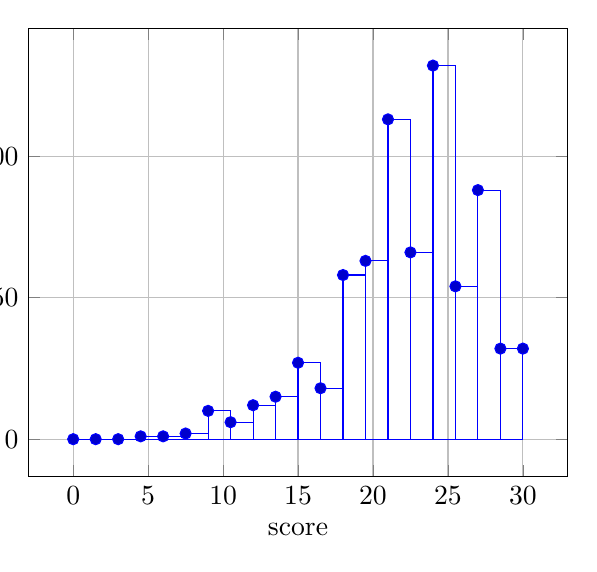
\begin{tikzpicture}
\begin{axis}[
xlabel={score},
ylabel={number of students},
ylabel style={overlay},
yticklabel style={overlay},
xmajorgrids=true,
ymajorgrids=true,
]
\addplot+[ybar interval] plot coordinates {
(0,0)
(1.5,0)
(3,0)
(4.5,1)
(6,1)
(7.5,2)
(9,10)
(10.5,6)
(12,12)
(13.5,15)
(15,27)
(16.5,18)
(18,58)
(19.5,63)
(21,113)
(22.5,66)
(24,132)
(25.5,54)
(27,88)
(28.5,32)
(30,32)
};
\end{axis}
\end{tikzpicture}
\end{center}
\vspace{8mm}
\begin{center}
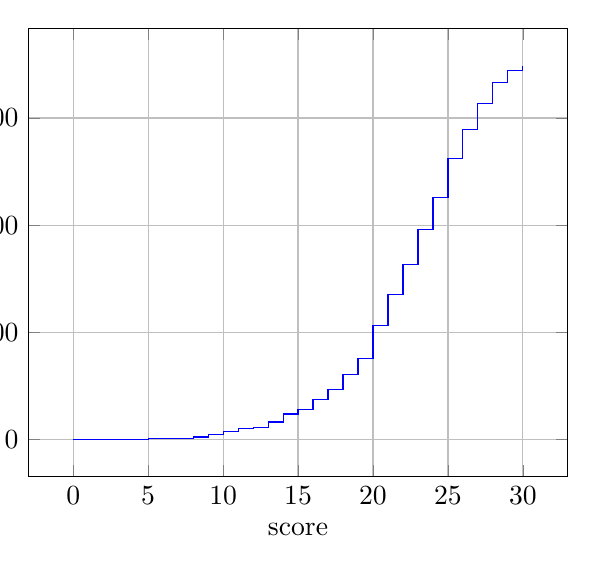
\begin{tikzpicture}
\begin{axis}[
xlabel={score},
ylabel={cumulative number of students},
ylabel style={overlay},
yticklabel style={overlay},
xmajorgrids=true,
ymajorgrids=true,
]
\addplot[const plot, draw=blue] coordinates {
(0,0)
(5,1)
(6,2)
(8,3)
(8,4)
(9,5)
(9,6)
(9,7)
(9,8)
(9,9)
(10,10)
(10,11)
(10,12)
(10,13)
(10,14)
(11,15)
(11,16)
(11,17)
(11,18)
(11,19)
(11,20)
(12,21)
(13,22)
(13,23)
(13,24)
(13,25)
(13,26)
(13,27)
(13,28)
(13,29)
(13,30)
(13,31)
(13,32)
(14,33)
(14,34)
(14,35)
(14,36)
(14,37)
(14,38)
(14,39)
(14,40)
(14,41)
(14,42)
(14,43)
(14,44)
(14,45)
(14,46)
(14,47)
(15,48)
(15,49)
(15,50)
(15,51)
(15,52)
(15,53)
(15,54)
(15,55)
(15,56)
(16,57)
(16,58)
(16,59)
(16,60)
(16,61)
(16,62)
(16,63)
(16,64)
(16,65)
(16,66)
(16,67)
(16,68)
(16,69)
(16,70)
(16,71)
(16,72)
(16,73)
(16,74)
(17,75)
(17,76)
(17,77)
(17,78)
(17,79)
(17,80)
(17,81)
(17,82)
(17,83)
(17,84)
(17,85)
(17,86)
(17,87)
(17,88)
(17,89)
(17,90)
(17,91)
(17,92)
(18,93)
(18,94)
(18,95)
(18,96)
(18,97)
(18,98)
(18,99)
(18,100)
(18,101)
(18,102)
(18,103)
(18,104)
(18,105)
(18,106)
(18,107)
(18,108)
(18,109)
(18,110)
(18,111)
(18,112)
(18,113)
(18,114)
(18,115)
(18,116)
(18,117)
(18,118)
(18,119)
(18,120)
(18,121)
(19,122)
(19,123)
(19,124)
(19,125)
(19,126)
(19,127)
(19,128)
(19,129)
(19,130)
(19,131)
(19,132)
(19,133)
(19,134)
(19,135)
(19,136)
(19,137)
(19,138)
(19,139)
(19,140)
(19,141)
(19,142)
(19,143)
(19,144)
(19,145)
(19,146)
(19,147)
(19,148)
(19,149)
(19,150)
(20,151)
(20,152)
(20,153)
(20,154)
(20,155)
(20,156)
(20,157)
(20,158)
(20,159)
(20,160)
(20,161)
(20,162)
(20,163)
(20,164)
(20,165)
(20,166)
(20,167)
(20,168)
(20,169)
(20,170)
(20,171)
(20,172)
(20,173)
(20,174)
(20,175)
(20,176)
(20,177)
(20,178)
(20,179)
(20,180)
(20,181)
(20,182)
(20,183)
(20,184)
(20,185)
(20,186)
(20,187)
(20,188)
(20,189)
(20,190)
(20,191)
(20,192)
(20,193)
(20,194)
(20,195)
(20,196)
(20,197)
(20,198)
(20,199)
(20,200)
(20,201)
(20,202)
(20,203)
(20,204)
(20,205)
(20,206)
(20,207)
(20,208)
(20,209)
(20,210)
(20,211)
(20,212)
(20,213)
(21,214)
(21,215)
(21,216)
(21,217)
(21,218)
(21,219)
(21,220)
(21,221)
(21,222)
(21,223)
(21,224)
(21,225)
(21,226)
(21,227)
(21,228)
(21,229)
(21,230)
(21,231)
(21,232)
(21,233)
(21,234)
(21,235)
(21,236)
(21,237)
(21,238)
(21,239)
(21,240)
(21,241)
(21,242)
(21,243)
(21,244)
(21,245)
(21,246)
(21,247)
(21,248)
(21,249)
(21,250)
(21,251)
(21,252)
(21,253)
(21,254)
(21,255)
(21,256)
(21,257)
(21,258)
(21,259)
(21,260)
(21,261)
(21,262)
(21,263)
(21,264)
(21,265)
(21,266)
(21,267)
(21,268)
(21,269)
(21,270)
(21,271)
(22,272)
(22,273)
(22,274)
(22,275)
(22,276)
(22,277)
(22,278)
(22,279)
(22,280)
(22,281)
(22,282)
(22,283)
(22,284)
(22,285)
(22,286)
(22,287)
(22,288)
(22,289)
(22,290)
(22,291)
(22,292)
(22,293)
(22,294)
(22,295)
(22,296)
(22,297)
(22,298)
(22,299)
(22,300)
(22,301)
(22,302)
(22,303)
(22,304)
(22,305)
(22,306)
(22,307)
(22,308)
(22,309)
(22,310)
(22,311)
(22,312)
(22,313)
(22,314)
(22,315)
(22,316)
(22,317)
(22,318)
(22,319)
(22,320)
(22,321)
(22,322)
(22,323)
(22,324)
(22,325)
(22,326)
(23,327)
(23,328)
(23,329)
(23,330)
(23,331)
(23,332)
(23,333)
(23,334)
(23,335)
(23,336)
(23,337)
(23,338)
(23,339)
(23,340)
(23,341)
(23,342)
(23,343)
(23,344)
(23,345)
(23,346)
(23,347)
(23,348)
(23,349)
(23,350)
(23,351)
(23,352)
(23,353)
(23,354)
(23,355)
(23,356)
(23,357)
(23,358)
(23,359)
(23,360)
(23,361)
(23,362)
(23,363)
(23,364)
(23,365)
(23,366)
(23,367)
(23,368)
(23,369)
(23,370)
(23,371)
(23,372)
(23,373)
(23,374)
(23,375)
(23,376)
(23,377)
(23,378)
(23,379)
(23,380)
(23,381)
(23,382)
(23,383)
(23,384)
(23,385)
(23,386)
(23,387)
(23,388)
(23,389)
(23,390)
(23,391)
(23,392)
(24,393)
(24,394)
(24,395)
(24,396)
(24,397)
(24,398)
(24,399)
(24,400)
(24,401)
(24,402)
(24,403)
(24,404)
(24,405)
(24,406)
(24,407)
(24,408)
(24,409)
(24,410)
(24,411)
(24,412)
(24,413)
(24,414)
(24,415)
(24,416)
(24,417)
(24,418)
(24,419)
(24,420)
(24,421)
(24,422)
(24,423)
(24,424)
(24,425)
(24,426)
(24,427)
(24,428)
(24,429)
(24,430)
(24,431)
(24,432)
(24,433)
(24,434)
(24,435)
(24,436)
(24,437)
(24,438)
(24,439)
(24,440)
(24,441)
(24,442)
(24,443)
(24,444)
(24,445)
(24,446)
(24,447)
(24,448)
(24,449)
(24,450)
(24,451)
(25,452)
(25,453)
(25,454)
(25,455)
(25,456)
(25,457)
(25,458)
(25,459)
(25,460)
(25,461)
(25,462)
(25,463)
(25,464)
(25,465)
(25,466)
(25,467)
(25,468)
(25,469)
(25,470)
(25,471)
(25,472)
(25,473)
(25,474)
(25,475)
(25,476)
(25,477)
(25,478)
(25,479)
(25,480)
(25,481)
(25,482)
(25,483)
(25,484)
(25,485)
(25,486)
(25,487)
(25,488)
(25,489)
(25,490)
(25,491)
(25,492)
(25,493)
(25,494)
(25,495)
(25,496)
(25,497)
(25,498)
(25,499)
(25,500)
(25,501)
(25,502)
(25,503)
(25,504)
(25,505)
(25,506)
(25,507)
(25,508)
(25,509)
(25,510)
(25,511)
(25,512)
(25,513)
(25,514)
(25,515)
(25,516)
(25,517)
(25,518)
(25,519)
(25,520)
(25,521)
(25,522)
(25,523)
(25,524)
(26,525)
(26,526)
(26,527)
(26,528)
(26,529)
(26,530)
(26,531)
(26,532)
(26,533)
(26,534)
(26,535)
(26,536)
(26,537)
(26,538)
(26,539)
(26,540)
(26,541)
(26,542)
(26,543)
(26,544)
(26,545)
(26,546)
(26,547)
(26,548)
(26,549)
(26,550)
(26,551)
(26,552)
(26,553)
(26,554)
(26,555)
(26,556)
(26,557)
(26,558)
(26,559)
(26,560)
(26,561)
(26,562)
(26,563)
(26,564)
(26,565)
(26,566)
(26,567)
(26,568)
(26,569)
(26,570)
(26,571)
(26,572)
(26,573)
(26,574)
(26,575)
(26,576)
(26,577)
(26,578)
(27,579)
(27,580)
(27,581)
(27,582)
(27,583)
(27,584)
(27,585)
(27,586)
(27,587)
(27,588)
(27,589)
(27,590)
(27,591)
(27,592)
(27,593)
(27,594)
(27,595)
(27,596)
(27,597)
(27,598)
(27,599)
(27,600)
(27,601)
(27,602)
(27,603)
(27,604)
(27,605)
(27,606)
(27,607)
(27,608)
(27,609)
(27,610)
(27,611)
(27,612)
(27,613)
(27,614)
(27,615)
(27,616)
(27,617)
(27,618)
(27,619)
(27,620)
(27,621)
(27,622)
(27,623)
(27,624)
(27,625)
(27,626)
(27,627)
(28,628)
(28,629)
(28,630)
(28,631)
(28,632)
(28,633)
(28,634)
(28,635)
(28,636)
(28,637)
(28,638)
(28,639)
(28,640)
(28,641)
(28,642)
(28,643)
(28,644)
(28,645)
(28,646)
(28,647)
(28,648)
(28,649)
(28,650)
(28,651)
(28,652)
(28,653)
(28,654)
(28,655)
(28,656)
(28,657)
(28,658)
(28,659)
(28,660)
(28,661)
(28,662)
(28,663)
(28,664)
(28,665)
(28,666)
(29,667)
(29,668)
(29,669)
(29,670)
(29,671)
(29,672)
(29,673)
(29,674)
(29,675)
(29,676)
(29,677)
(29,678)
(29,679)
(29,680)
(29,681)
(29,682)
(29,683)
(29,684)
(29,685)
(29,686)
(29,687)
(29,688)
(30,689)
(30,690)
(30,691)
(30,692)
(30,693)
(30,694)
(30,695)
(30,696)
(30,697)
(30,698)
(30,698)
};
\end{axis}
\end{tikzpicture}
\end{center}

\clearpage
\section{Question summary data}

The plot below shows the \emph{difficulty} and \emph{discrimination}
for each question. Ideally the discrimination should be high, and
there should be a mixture of easy and hard questions.

\begin{center}
\begin{tabular}{lll}
quantity & symbol & description \\
\hline
difficulty & $D_{\rm Q}(Q)$ & fraction of students who get question $Q$ incorrect \\
discrimination & $r^{\rm P}_{\rm Q}(Q)$ & correlation of scores between question $Q$ and the total exam
\end{tabular}
\end{center}

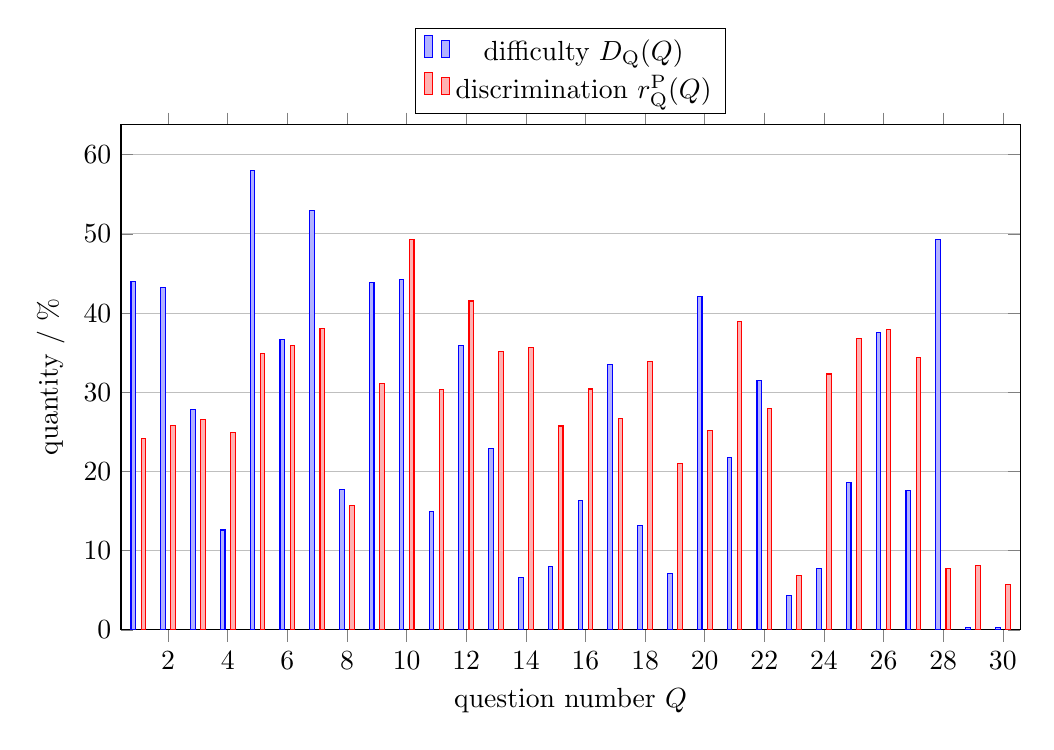
\begin{tikzpicture}
\begin{axis}[
ybar, ymin=0,
xmin=1, xmax=30,
width=13cm, height=8cm,
xlabel={question number $Q$},
ylabel={quantity / \%},
ymajorgrids=true,
enlarge x limits=0.02,
legend style={at={(0.5,1.02)},anchor=south},
bar width=0.0583333cm,
]
\addplot coordinates {
(1,43.9828)
(2,43.2665)
(3,27.7937)
(4,12.6074)
(5,58.0229)
(6,36.6762)
(7,53.0086)
(8,17.765)
(9,43.8395)
(10,44.2693)
(11,14.8997)
(12,35.9599)
(13,22.9226)
(14,6.59026)
(15,8.02292)
(16,16.3324)
(17,33.5244)
(18,13.1805)
(19,7.16332)
(20,42.1203)
(21,21.7765)
(22,31.5186)
(23,4.29799)
(24,7.73639)
(25,18.6246)
(26,37.5358)
(27,17.6218)
(28,49.2837)
(29,0.286533)
(30,0.286533)
};
\addplot coordinates {
(1,24.1244)
(2,25.839)
(3,26.547)
(4,24.9014)
(5,34.8702)
(6,35.8846)
(7,38.0735)
(8,15.7523)
(9,31.1292)
(10,49.2523)
(11,30.3196)
(12,41.5297)
(13,35.2016)
(14,35.6618)
(15,25.7469)
(16,30.4092)
(17,26.7393)
(18,33.9238)
(19,20.9969)
(20,25.1524)
(21,38.9571)
(22,27.963)
(23,6.84625)
(24,32.3083)
(25,36.8135)
(26,37.9041)
(27,34.4031)
(28,7.74044)
(29,8.18009)
(30,5.77028)
};
\legend{difficulty $D_{\rm Q}(Q)$,discrimination $r^{\rm P}_{\rm Q}(Q)$};
\end{axis}
\end{tikzpicture}


\vspace{1em}

The following plot shows the relative points for the question
variants. Variants with $R_{\rm QV}(Q,V)$ above 100\% are easier than
average (more points awarded), while values below 100\% indicate
a harder-than-average variant.

\vspace{1em}

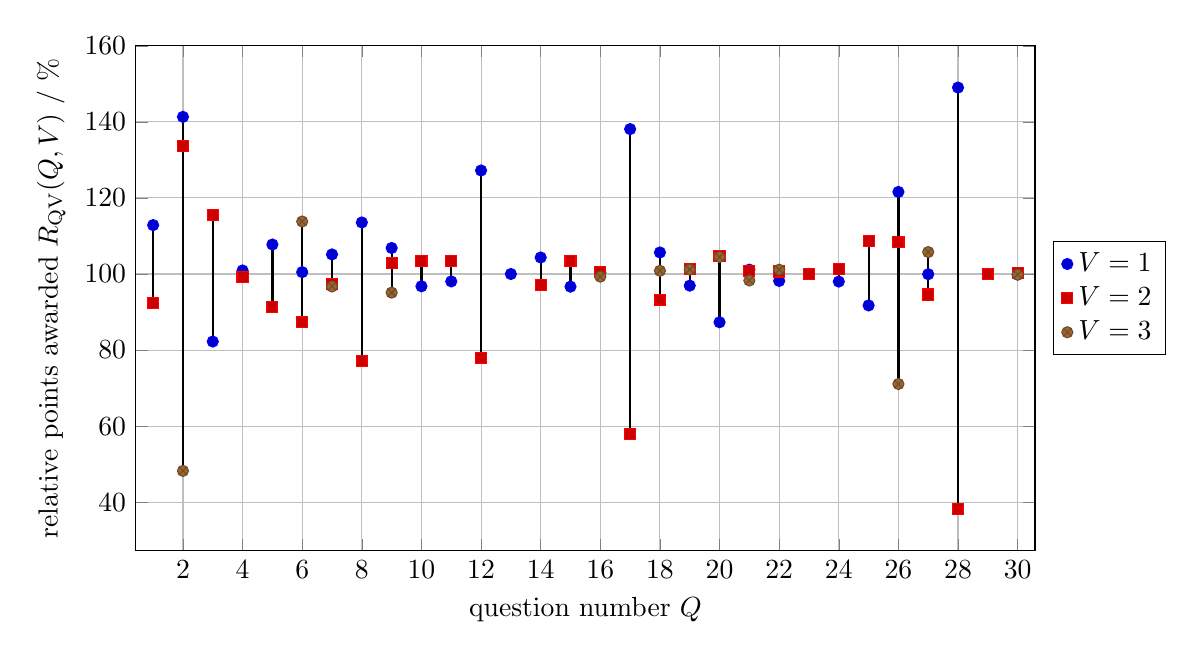
\begin{tikzpicture}
\begin{axis}[
xmin=1, xmax=30,
width=13cm, height=8cm,
ylabel={relative points awarded $R_{\rm QV}(Q,V)$ / \%},
xlabel={question number $Q$},
xmajorgrids=true,
ymajorgrids=true,
enlarge x limits=0.02,
legend style={at={(1.02,0.5)},anchor=west},
]
\addplot[mark=none,draw=black,thick,forget plot] coordinates {
(1,92.3221)
(1,112.855)
};
\addplot[mark=none,draw=black,thick,forget plot] coordinates {
(2,48.234)
(2,141.314)
};
\addplot[mark=none,draw=black,thick,forget plot] coordinates {
(3,82.243)
(3,115.472)
};
\addplot[mark=none,draw=black,thick,forget plot] coordinates {
(4,99.21)
(4,100.923)
};
\addplot[mark=none,draw=black,thick,forget plot] coordinates {
(5,91.4036)
(5,107.753)
};
\addplot[mark=none,draw=black,thick,forget plot] coordinates {
(6,87.2859)
(6,113.804)
};
\addplot[mark=none,draw=black,thick,forget plot] coordinates {
(7,96.7295)
(7,105.151)
};
\addplot[mark=none,draw=black,thick,forget plot] coordinates {
(8,77.171)
(8,113.551)
};
\addplot[mark=none,draw=black,thick,forget plot] coordinates {
(9,95.1069)
(9,106.837)
};
\addplot[mark=none,draw=black,thick,forget plot] coordinates {
(10,96.7736)
(10,103.358)
};
\addplot[mark=none,draw=black,thick,forget plot] coordinates {
(11,98.0551)
(11,103.464)
};
\addplot[mark=none,draw=black,thick,forget plot] coordinates {
(12,77.8733)
(12,127.217)
};
\addplot[mark=none,draw=black,thick,forget plot] coordinates {
(14,97.1615)
(14,104.34)
};
\addplot[mark=none,draw=black,thick,forget plot] coordinates {
(15,96.6768)
(15,103.381)
};
\addplot[mark=none,draw=black,thick,forget plot] coordinates {
(16,99.3075)
(16,100.506)
};
\addplot[mark=none,draw=black,thick,forget plot] coordinates {
(17,57.9975)
(17,138.101)
};
\addplot[mark=none,draw=black,thick,forget plot] coordinates {
(18,93.0919)
(18,105.667)
};
\addplot[mark=none,draw=black,thick,forget plot] coordinates {
(19,96.9444)
(19,101.293)
};
\addplot[mark=none,draw=black,thick,forget plot] coordinates {
(20,87.315)
(20,104.731)
};
\addplot[mark=none,draw=black,thick,forget plot] coordinates {
(21,98.2962)
(21,101.147)
};
\addplot[mark=none,draw=black,thick,forget plot] coordinates {
(22,98.1786)
(22,101.138)
};
\addplot[mark=none,draw=black,thick,forget plot] coordinates {
(23,99.9711)
(23,100.037)
};
\addplot[mark=none,draw=black,thick,forget plot] coordinates {
(24,98.0078)
(24,101.35)
};
\addplot[mark=none,draw=black,thick,forget plot] coordinates {
(25,91.7376)
(25,108.75)
};
\addplot[mark=none,draw=black,thick,forget plot] coordinates {
(26,71.0752)
(26,121.579)
};
\addplot[mark=none,draw=black,thick,forget plot] coordinates {
(27,94.6054)
(27,105.767)
};
\addplot[mark=none,draw=black,thick,forget plot] coordinates {
(28,38.2864)
(28,149.022)
};
\addplot[mark=none,draw=black,thick,forget plot] coordinates {
(29,99.9585)
(29,100.032)
};
\addplot[mark=none,draw=black,thick,forget plot] coordinates {
(30,99.8436)
(30,100.287)
};
\addplot+[only marks] coordinates {
(1,112.855)
(2,141.314)
(3,82.243)
(4,100.923)
(5,107.753)
(6,100.494)
(7,105.151)
(8,113.551)
(9,106.837)
(10,96.7736)
(11,98.0551)
(12,127.217)
(13,100)
(14,104.34)
(15,96.6768)
(16,100.374)
(17,138.101)
(18,105.667)
(19,96.9444)
(20,87.315)
(21,101.147)
(22,98.1786)
(23,100.037)
(24,98.0078)
(25,91.7376)
(26,121.579)
(27,99.9441)
(28,149.022)
(29,100.032)
(30,99.8475)
};
\addplot+[only marks] coordinates {
(1,92.3221)
(2,133.752)
(3,115.472)
(4,99.21)
(5,91.4036)
(6,87.2859)
(7,97.4032)
(8,77.171)
(9,102.955)
(10,103.358)
(11,103.464)
(12,77.8733)
(14,97.1615)
(15,103.381)
(16,100.506)
(17,57.9975)
(18,93.0919)
(19,101.293)
(20,104.731)
(21,100.708)
(22,100.658)
(23,99.9711)
(24,101.35)
(25,108.75)
(26,108.409)
(27,94.6054)
(28,38.2864)
(29,99.9585)
(30,100.287)
};
\addplot+[only marks] coordinates {
(2,48.234)
(6,113.804)
(7,96.7295)
(9,95.1069)
(16,99.3075)
(18,100.842)
(19,101.176)
(20,104.483)
(21,98.2962)
(22,101.138)
(26,71.0752)
(27,105.767)
(30,99.8436)
};
\legend{$V = 1$,$V = 2$,$V = 3$};
\end{axis}
\end{tikzpicture}


\clearpage

The scatter-plot below contains the same information as the first plot
in this section, but plots the \emph{discrimination} against the
\emph{difficulty} for each question. Questions should ideally be high
on this plot (discriminating well), and there should be a mixture of
left-to-right (difficulty) values.

\vspace{2em}

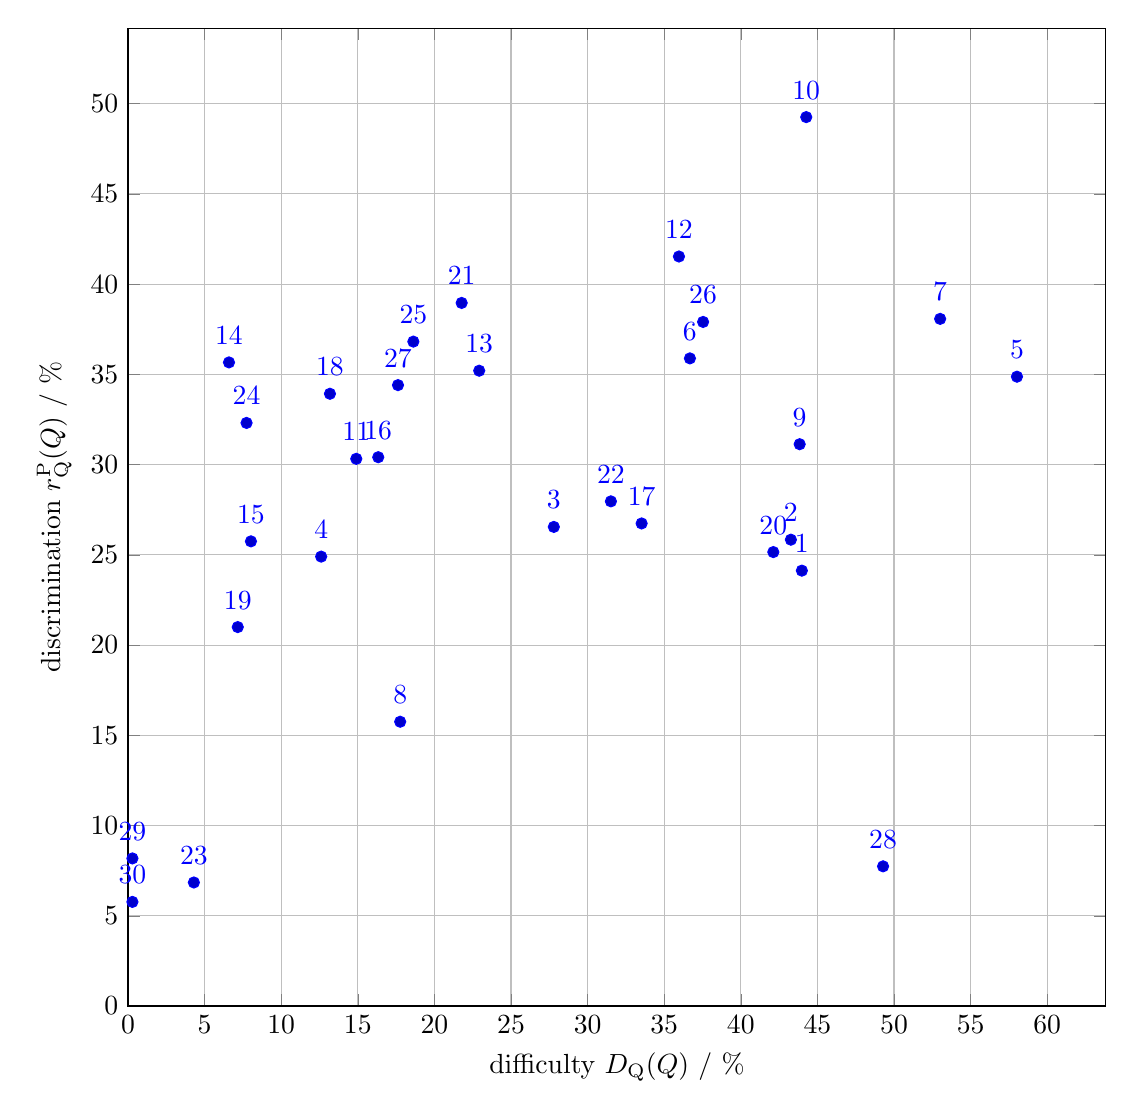
\begin{tikzpicture}
\begin{axis}[
xmin=0, ymin=0,
width=14cm, height=14cm,
only marks,
xlabel={difficulty $D_{\rm Q}(Q)$ / \%},
ylabel={discrimination $r^{\rm P}_{\rm Q}(Q)$ / \%},
xmajorgrids=true,
ymajorgrids=true,
nodes near coords,
point meta=explicit symbolic,
every node near coord/.style={yshift=3},
]
\addplot coordinates {
(43.9828,24.1244) [1]
(43.2665,25.839) [2]
(27.7937,26.547) [3]
(12.6074,24.9014) [4]
(58.0229,34.8702) [5]
(36.6762,35.8846) [6]
(53.0086,38.0735) [7]
(17.765,15.7523) [8]
(43.8395,31.1292) [9]
(44.2693,49.2523) [10]
(14.8997,30.3196) [11]
(35.9599,41.5297) [12]
(22.9226,35.2016) [13]
(6.59026,35.6618) [14]
(8.02292,25.7469) [15]
(16.3324,30.4092) [16]
(33.5244,26.7393) [17]
(13.1805,33.9238) [18]
(7.16332,20.9969) [19]
(42.1203,25.1524) [20]
(21.7765,38.9571) [21]
(31.5186,27.963) [22]
(4.29799,6.84625) [23]
(7.73639,32.3083) [24]
(18.6246,36.8135) [25]
(37.5358,37.9041) [26]
(17.6218,34.4031) [27]
(49.2837,7.74044) [28]
(0.286533,8.18009) [29]
(0.286533,5.77028) [30]
};
\end{axis}
\end{tikzpicture}


\clearpage

The plot below shows the correlation coefficient $r^{\rm s}_{\rm QQ}$
of student scores on different questions. Positive correlations are
shown in red colors, and negative correlations in blue. Gray color
indicates uncorrelated questions. Each question correlates perfectly
with itself ($r = 1$), but self-correlations are plotted as $r = 0$ to
improve the colorbar range.

\vspace{2em}

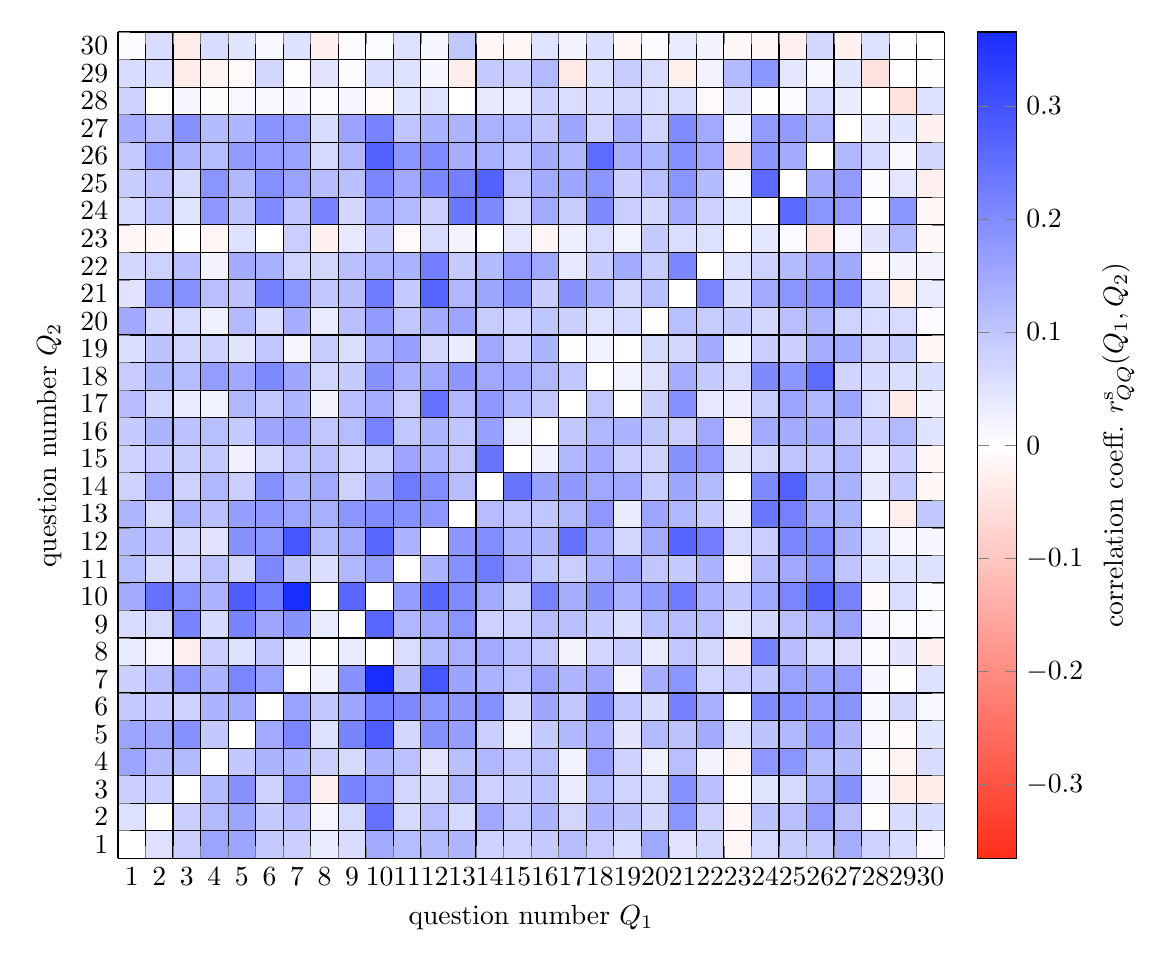
\begin{tikzpicture}
\begin{axis}[
view={0}{90},
width=14cm,
axis equal image,
xlabel={question number $Q_1$},
ylabel={question number $Q_2$},
colorbar,
x tick label as interval,
y tick label as interval,
xtick=data,
ytick=data,
point meta max=0.365262,
point meta min=-0.365262,
colormap={RdBl}{rgb255=(255,45,25) color=(white) rgb255=(25,45,255)},
colorbar style={
  ylabel={correlation coeff. $r^{\rm s}_{QQ}(Q_1,Q_2)$},
  every axis y label/.style=
  {at={(ticklabel cs:0.5)},rotate=90,anchor=near ticklabel},
  },
]
\addplot3[surf,shader=flat corner,draw=black] coordinates {
(1,1,0) (2,1,0.0534327) (3,1,0.0816532) (4,1,0.159084) (5,1,0.157144) (6,1,0.0922573) (7,1,0.0824878) (8,1,0.0336895) (9,1,0.0605694) (10,1,0.145814) (11,1,0.115569) (12,1,0.117905) (13,1,0.127909) (14,1,0.0787317) (15,1,0.0783036) (16,1,0.0925996) (17,1,0.116658) (18,1,0.0898951) (19,1,0.0560585) (20,1,0.150178) (21,1,0.0499748) (22,1,0.069816) (23,1,-0.0170043) (24,1,0.0675131) (25,1,0.0876508) (26,1,0.0939721) (27,1,0.143186) (28,1,0.079088) (29,1,0.0604964) (30,1,0.00649834) (31,1,0)

(1,2,0.0534327) (2,2,0) (3,2,0.0843203) (4,2,0.121313) (5,2,0.156857) (6,2,0.0914316) (7,2,0.115379) (8,2,0.0177757) (9,2,0.0676286) (10,2,0.246297) (11,2,0.064989) (12,2,0.110881) (13,2,0.0672372) (14,2,0.152647) (15,2,0.0933643) (16,2,0.13045) (17,2,0.0720134) (18,2,0.129888) (19,2,0.105032) (20,2,0.0690869) (21,2,0.183809) (22,2,0.0797545) (23,2,-0.0139719) (24,2,0.104296) (25,2,0.109586) (26,2,0.171045) (27,2,0.112191) (28,2,-0.00483928) (29,2,0.0613839) (30,2,0.0613839) (31,2,0)

(1,3,0.0816532) (2,3,0.0843203) (3,3,0) (4,3,0.120833) (5,3,0.190744) (6,3,0.0786246) (7,3,0.180462) (8,3,-0.028985) (9,3,0.212377) (10,3,0.193912) (11,3,0.072698) (12,3,0.068227) (13,3,0.133374) (14,3,0.080107) (15,3,0.0875366) (16,3,0.106542) (17,3,0.0336198) (18,3,0.11751) (19,3,0.0756869) (20,3,0.066626) (21,3,0.191805) (22,3,0.109131) (23,3,-0.00533147) (24,3,0.0477777) (25,3,0.0646351) (26,3,0.126679) (27,3,0.191492) (28,3,0.0152862) (29,3,-0.033258) (30,3,-0.033258) (31,3,0)

(1,4,0.159084) (2,4,0.121313) (3,4,0.120833) (4,4,0) (5,4,0.095675) (6,4,0.131878) (7,4,0.132767) (8,4,0.0831877) (9,4,0.0645535) (10,4,0.130716) (11,4,0.107735) (12,4,0.0481662) (13,4,0.111186) (14,4,0.12526) (15,4,0.094376) (16,4,0.11241) (17,4,0.0228441) (18,4,0.170986) (19,4,0.0786014) (20,4,0.0256483) (21,4,0.113325) (22,4,0.0210293) (23,4,-0.0166471) (24,4,0.180807) (25,4,0.184154) (26,4,0.115596) (27,4,0.118865) (28,4,0.00544209) (29,4,-0.0203604) (30,4,0.0603872) (31,4,0)

(1,5,0.157144) (2,5,0.156857) (3,5,0.190744) (4,5,0.095675) (5,5,0) (6,5,0.147348) (7,5,0.211225) (8,5,0.0535567) (9,5,0.213249) (10,5,0.284676) (11,5,0.0705683) (12,5,0.18972) (13,5,0.166878) (14,5,0.0855217) (15,5,0.0267926) (16,5,0.0930884) (17,5,0.124378) (18,5,0.151197) (19,5,0.0448989) (20,5,0.120013) (21,5,0.104133) (22,5,0.145897) (23,5,0.0514301) (24,5,0.105045) (25,5,0.123559) (26,5,0.173739) (27,5,0.126721) (28,5,0.0139422) (29,5,-0.00871439) (30,5,0.0455949) (31,5,0)

(1,6,0.0922573) (2,6,0.0914316) (3,6,0.0786246) (4,6,0.131878) (5,6,0.147348) (6,6,0) (7,6,0.162599) (8,6,0.0973898) (9,6,0.1544) (10,6,0.225461) (11,6,0.207519) (12,6,0.185492) (13,6,0.179062) (14,6,0.193254) (15,6,0.0707105) (16,6,0.154319) (17,6,0.0955789) (18,6,0.204392) (19,6,0.0998538) (20,6,0.0612439) (21,6,0.217903) (22,6,0.136373) (23,6,-4.20001e-05) (24,6,0.202457) (25,6,0.193356) (26,6,0.171342) (27,6,0.18639) (28,6,0.0109043) (29,6,0.0704371) (30,6,0.0148205) (31,6,0)

(1,7,0.0824878) (2,7,0.115379) (3,7,0.180462) (4,7,0.132767) (5,7,0.211225) (6,7,0.162599) (7,7,0) (8,7,0.0245534) (9,7,0.189716) (10,7,0.365262) (11,7,0.103758) (12,7,0.292796) (13,7,0.158342) (14,7,0.134392) (15,7,0.109002) (16,7,0.159734) (17,7,0.12745) (18,7,0.154712) (19,7,0.0166491) (20,7,0.140429) (21,7,0.1838) (22,7,0.0764982) (23,7,0.0863008) (24,7,0.100732) (25,7,0.162871) (26,7,0.160758) (27,7,0.171773) (28,7,0.0152178) (29,7,-0.00323141) (30,7,0.0504715) (31,7,0)

(1,8,0.0336895) (2,8,0.0177757) (3,8,-0.028985) (4,8,0.0831877) (5,8,0.0535567) (6,8,0.0973898) (7,8,0.0245534) (8,8,0) (9,8,0.0350434) (10,8,0.000800039) (11,8,0.0581514) (12,8,0.120363) (13,8,0.138897) (14,8,0.148475) (15,8,0.111098) (16,8,0.0988413) (17,8,0.0192927) (18,8,0.0737534) (19,8,0.0889178) (20,8,0.0362171) (21,8,0.0998735) (22,8,0.0719412) (23,8,-0.0245715) (24,8,0.216154) (25,8,0.114627) (26,8,0.0654544) (27,8,0.0604932) (28,8,0.00665954) (29,8,0.0452091) (30,8,-0.0249153) (31,8,0)

(1,9,0.0605694) (2,9,0.0676286) (3,9,0.212377) (4,9,0.0645535) (5,9,0.213249) (6,9,0.1544) (7,9,0.189716) (8,9,0.0350434) (9,9,0) (10,9,0.264698) (11,9,0.124927) (12,9,0.150194) (13,9,0.184482) (14,9,0.0795265) (15,9,0.0791841) (16,9,0.11734) (17,9,0.112634) (18,9,0.0910519) (19,9,0.0568804) (20,9,0.11176) (21,9,0.114478) (22,9,0.109088) (23,9,0.0405475) (24,9,0.0683731) (25,9,0.111313) (26,9,0.126058) (27,9,0.159728) (28,9,0.0184345) (29,9,0.00665541) (30,9,0.00665541) (31,9,0)

(1,10,0.145814) (2,10,0.246297) (3,10,0.193912) (4,10,0.130716) (5,10,0.284676) (6,10,0.225461) (7,10,0.365262) (8,10,0.000800039) (9,10,0.264698) (10,10,0) (11,10,0.169778) (12,10,0.263765) (13,10,0.200158) (14,10,0.146897) (15,10,0.0871644) (16,10,0.21483) (17,10,0.143031) (18,10,0.189904) (19,10,0.132712) (20,10,0.174363) (21,10,0.228598) (22,10,0.134147) (23,10,0.0955586) (24,10,0.152164) (25,10,0.210783) (26,10,0.274095) (27,10,0.216123) (28,10,-0.00742235) (29,10,0.0601459) (30,10,0.00618467) (31,10,0)

(1,11,0.115569) (2,11,0.064989) (3,11,0.072698) (4,11,0.107735) (5,11,0.0705683) (6,11,0.207519) (7,11,0.103758) (8,11,0.0581514) (9,11,0.124927) (10,11,0.169778) (11,11,0) (12,11,0.130806) (13,11,0.192972) (14,11,0.229393) (15,11,0.157828) (16,11,0.0981115) (17,11,0.086375) (18,11,0.134306) (19,11,0.164601) (20,11,0.0993705) (21,11,0.09117) (22,11,0.131811) (23,11,-0.00932213) (24,11,0.119784) (25,11,0.151201) (26,11,0.18249) (27,11,0.102149) (28,11,0.0462332) (29,11,0.0528405) (30,11,0.0528405) (31,11,0)

(1,12,0.117905) (2,12,0.110881) (3,12,0.068227) (4,12,0.0481662) (5,12,0.18972) (6,12,0.185492) (7,12,0.292796) (8,12,0.120363) (9,12,0.150194) (10,12,0.263765) (11,12,0.130806) (12,12,0) (13,12,0.18086) (14,12,0.198039) (15,12,0.13037) (16,12,0.129265) (17,12,0.245715) (18,12,0.149299) (19,12,0.0696936) (20,12,0.146795) (21,12,0.270105) (22,12,0.224191) (23,12,0.0620023) (24,12,0.0847207) (25,12,0.208987) (26,12,0.202138) (27,12,0.1314) (28,12,0.0495515) (29,12,0.0156836) (30,12,0.0156836) (31,12,0)

(1,13,0.127909) (2,13,0.0672372) (3,13,0.133374) (4,13,0.111186) (5,13,0.166878) (6,13,0.179062) (7,13,0.158342) (8,13,0.138897) (9,13,0.184482) (10,13,0.200158) (11,13,0.192972) (12,13,0.18086) (13,13,0) (14,13,0.116157) (15,13,0.102426) (16,13,0.100208) (17,13,0.125347) (18,13,0.180467) (19,13,0.0335537) (20,13,0.15606) (21,13,0.125175) (22,13,0.0922192) (23,13,0.0188763) (24,13,0.237567) (25,13,0.220632) (26,13,0.140376) (27,13,0.132444) (28,13,0.00099625) (29,13,-0.0292334) (30,13,0.0982973) (31,13,0)

(1,14,0.0787317) (2,14,0.152647) (3,14,0.080107) (4,14,0.12526) (5,14,0.0855217) (6,14,0.193254) (7,14,0.134392) (8,14,0.148475) (9,14,0.0795265) (10,14,0.146897) (11,14,0.229393) (12,14,0.198039) (13,14,0.116157) (14,14,0) (15,14,0.240399) (16,14,0.163813) (17,14,0.178323) (18,14,0.15255) (19,14,0.150131) (20,14,0.0891678) (21,14,0.153655) (22,14,0.118091) (23,14,0.000652632) (24,14,0.204053) (25,14,0.273398) (26,14,0.139922) (27,14,0.134792) (28,14,0.038455) (29,14,0.0937887) (30,14,-0.0142385) (31,14,0)

(1,15,0.0783036) (2,15,0.0933643) (3,15,0.0875366) (4,15,0.094376) (5,15,0.0267926) (6,15,0.0707105) (7,15,0.109002) (8,15,0.111098) (9,15,0.0791841) (10,15,0.0871644) (11,15,0.157828) (12,15,0.13037) (13,15,0.102426) (14,15,0.240399) (15,15,0) (16,15,0.0264493) (17,15,0.12542) (18,15,0.149965) (19,15,0.0815709) (20,15,0.0791773) (21,15,0.189186) (22,15,0.174247) (23,15,0.041428) (24,15,0.0724) (25,15,0.102555) (26,15,0.0978078) (27,15,0.126405) (28,15,0.0358788) (29,15,0.0828355) (30,15,-0.015832) (31,15,0)

(1,16,0.0925996) (2,16,0.13045) (3,16,0.106542) (4,16,0.11241) (5,16,0.0930884) (6,16,0.154319) (7,16,0.159734) (8,16,0.0988413) (9,16,0.11734) (10,16,0.21483) (11,16,0.0981115) (12,16,0.129265) (13,16,0.100208) (14,16,0.163813) (15,16,0.0264493) (16,16,0) (17,16,0.0967291) (18,16,0.12573) (19,16,0.132762) (20,16,0.101906) (21,16,0.0861538) (22,16,0.15073) (23,16,-0.017193) (24,16,0.147682) (25,16,0.147018) (26,16,0.145745) (27,16,0.100817) (28,16,0.0838508) (29,16,0.121329) (30,16,0.0488224) (31,16,0)

(1,17,0.116658) (2,17,0.0720134) (3,17,0.0336198) (4,17,0.0228441) (5,17,0.124378) (6,17,0.0955789) (7,17,0.12745) (8,17,0.0192927) (9,17,0.112634) (10,17,0.143031) (11,17,0.086375) (12,17,0.245715) (13,17,0.125347) (14,17,0.178323) (15,17,0.12542) (16,17,0.0967291) (17,17,0) (18,17,0.100099) (19,17,0.00279878) (20,17,0.0825984) (21,17,0.191497) (22,17,0.0408032) (23,17,0.0290699) (24,17,0.0897021) (25,17,0.159171) (26,17,0.126392) (27,17,0.157434) (28,17,0.0587372) (29,17,-0.0380679) (30,17,0.0187086) (31,17,0)

(1,18,0.0898951) (2,18,0.129888) (3,18,0.11751) (4,18,0.170986) (5,18,0.151197) (6,18,0.204392) (7,18,0.154712) (8,18,0.0737534) (9,18,0.0910519) (10,18,0.189904) (11,18,0.134306) (12,18,0.149299) (13,18,0.180467) (14,18,0.15255) (15,18,0.149965) (16,18,0.12573) (17,18,0.100099) (18,18,0) (19,18,0.0231522) (20,18,0.0536032) (21,18,0.143307) (22,18,0.0911852) (23,18,0.063604) (24,18,0.204214) (25,18,0.183474) (26,18,0.257732) (27,18,0.0754533) (28,18,0.0648811) (29,18,0.0583463) (30,18,0.0583463) (31,18,0)

(1,19,0.0560585) (2,19,0.105032) (3,19,0.0756869) (4,19,0.0786014) (5,19,0.0448989) (6,19,0.0998538) (7,19,0.0166491) (8,19,0.0889178) (9,19,0.0568804) (10,19,0.132712) (11,19,0.164601) (12,19,0.0696936) (13,19,0.0335537) (14,19,0.150131) (15,19,0.0815709) (16,19,0.132762) (17,19,0.00279878) (18,19,0.0231522) (19,19,0) (20,19,0.0668332) (21,19,0.0688073) (22,19,0.146374) (23,19,0.0233112) (24,19,0.0859178) (25,19,0.0811656) (26,19,0.140343) (27,19,0.148571) (28,19,0.0706535) (29,19,0.0890449) (30,19,-0.0148905) (31,19,0)

(1,20,0.150178) (2,20,0.0690869) (3,20,0.066626) (4,20,0.0256483) (5,20,0.120013) (6,20,0.0612439) (7,20,0.140429) (8,20,0.0362171) (9,20,0.11176) (10,20,0.174363) (11,20,0.0993705) (12,20,0.146795) (13,20,0.15606) (14,20,0.0891678) (15,20,0.0791773) (16,20,0.101906) (17,20,0.0825984) (18,20,0.0536032) (19,20,0.0668332) (20,20,0) (21,20,0.112323) (22,20,0.0895305) (23,20,0.0910469) (24,20,0.0679328) (25,20,0.113614) (26,20,0.129703) (27,20,0.0776181) (28,20,0.058653) (29,20,0.0628387) (30,20,0.00855478) (31,20,0)

(1,21,0.0499748) (2,21,0.183809) (3,21,0.191805) (4,21,0.113325) (5,21,0.104133) (6,21,0.217903) (7,21,0.1838) (8,21,0.0998735) (9,21,0.114478) (10,21,0.228598) (11,21,0.09117) (12,21,0.270105) (13,21,0.125175) (14,21,0.153655) (15,21,0.189186) (16,21,0.0861538) (17,21,0.191497) (18,21,0.143307) (19,21,0.0688073) (20,21,0.112323) (21,21,0) (22,21,0.209889) (23,21,0.0593401) (24,21,0.146046) (25,21,0.184486) (26,21,0.193166) (27,21,0.202393) (28,21,0.0631051) (29,21,-0.0282837) (30,21,0.0366571) (31,21,0)

(1,22,0.069816) (2,22,0.0797545) (3,22,0.109131) (4,22,0.0210293) (5,22,0.145897) (6,22,0.136373) (7,22,0.0764982) (8,22,0.0719412) (9,22,0.109088) (10,22,0.134147) (11,22,0.131811) (12,22,0.224191) (13,22,0.0922192) (14,22,0.118091) (15,22,0.174247) (16,22,0.15073) (17,22,0.0408032) (18,22,0.0911852) (19,22,0.146374) (20,22,0.0895305) (21,22,0.209889) (22,22,0) (23,22,0.0538922) (24,22,0.0805642) (25,22,0.11902) (26,22,0.149158) (27,22,0.147564) (28,22,-0.00878376) (29,22,0.0213243) (30,22,0.0213243) (31,22,0)

(1,23,-0.0170043) (2,23,-0.0139719) (3,23,-0.00533147) (4,23,-0.0166471) (5,23,0.0514301) (6,23,-4.20001e-05) (7,23,0.0863008) (8,23,-0.0245715) (9,23,0.0405475) (10,23,0.0955586) (11,23,-0.00932213) (12,23,0.0620023) (13,23,0.0188763) (14,23,0.000652632) (15,23,0.041428) (16,23,-0.017193) (17,23,0.0290699) (18,23,0.063604) (19,23,0.0233112) (20,23,0.0910469) (21,23,0.0593401) (22,23,0.0538922) (23,23,0) (24,23,0.0443955) (25,23,0.00748683) (26,23,-0.0475696) (27,23,0.013228) (28,23,0.0454248) (29,23,0.120796) (30,23,-0.0113601) (31,23,0)

(1,24,0.0675131) (2,24,0.104296) (3,24,0.0477777) (4,24,0.180807) (5,24,0.105045) (6,24,0.202457) (7,24,0.100732) (8,24,0.216154) (9,24,0.0683731) (10,24,0.152164) (11,24,0.119784) (12,24,0.0847207) (13,24,0.237567) (14,24,0.204053) (15,24,0.0724) (16,24,0.147682) (17,24,0.0897021) (18,24,0.204214) (19,24,0.0859178) (20,24,0.0679328) (21,24,0.146046) (22,24,0.0805642) (23,24,0.0443955) (24,24,0) (25,24,0.260922) (26,24,0.185283) (27,24,0.175708) (28,24,0.004149) (29,24,0.185121) (30,24,-0.0155226) (31,24,0)

(1,25,0.0876508) (2,25,0.109586) (3,25,0.0646351) (4,25,0.184154) (5,25,0.123559) (6,25,0.193356) (7,25,0.162871) (8,25,0.114627) (9,25,0.111313) (10,25,0.210783) (11,25,0.151201) (12,25,0.208987) (13,25,0.220632) (14,25,0.273398) (15,25,0.102555) (16,25,0.147018) (17,25,0.159171) (18,25,0.183474) (19,25,0.0811656) (20,25,0.113614) (21,25,0.184486) (22,25,0.11902) (23,25,0.00748683) (24,25,0.260922) (25,25,0) (26,25,0.145947) (27,25,0.174744) (28,25,0.00685467) (29,25,0.0432025) (30,25,-0.0256453) (31,25,0)

(1,26,0.0939721) (2,26,0.171045) (3,26,0.126679) (4,26,0.115596) (5,26,0.173739) (6,26,0.171342) (7,26,0.160758) (8,26,0.0654544) (9,26,0.126058) (10,26,0.274095) (11,26,0.18249) (12,26,0.202138) (13,26,0.140376) (14,26,0.139922) (15,26,0.0978078) (16,26,0.145745) (17,26,0.126392) (18,26,0.257732) (19,26,0.140343) (20,26,0.129703) (21,26,0.193166) (22,26,0.149158) (23,26,-0.0475696) (24,26,0.185283) (25,26,0.145947) (26,26,0) (27,26,0.122937) (28,26,0.0643697) (29,26,0.0137986) (30,26,0.0691517) (31,26,0)

(1,27,0.143186) (2,27,0.112191) (3,27,0.191492) (4,27,0.118865) (5,27,0.126721) (6,27,0.18639) (7,27,0.171773) (8,27,0.0604932) (9,27,0.159728) (10,27,0.216123) (11,27,0.102149) (12,27,0.1314) (13,27,0.132444) (14,27,0.134792) (15,27,0.126405) (16,27,0.100817) (17,27,0.157434) (18,27,0.0754533) (19,27,0.148571) (20,27,0.0776181) (21,27,0.202393) (22,27,0.147564) (23,27,0.013228) (24,27,0.175708) (25,27,0.174744) (26,27,0.122937) (27,27,0) (28,27,0.0329511) (29,27,0.0455546) (30,27,-0.024793) (31,27,0)

(1,28,0.079088) (2,28,-0.00483928) (3,28,0.0152862) (4,28,0.00544209) (5,28,0.0139422) (6,28,0.0109043) (7,28,0.0152178) (8,28,0.00665954) (9,28,0.0184345) (10,28,-0.00742235) (11,28,0.0462332) (12,28,0.0495515) (13,28,0.00099625) (14,28,0.038455) (15,28,0.0358788) (16,28,0.0838508) (17,28,0.0587372) (18,28,0.0648811) (19,28,0.0706535) (20,28,0.058653) (21,28,0.0631051) (22,28,-0.00878376) (23,28,0.0454248) (24,28,0.004149) (25,28,0.00685467) (26,28,0.0643697) (27,28,0.0329511) (28,28,0) (29,28,-0.0528431) (30,28,0.0543792) (31,28,0)

(1,29,0.0604964) (2,29,0.0613839) (3,29,-0.033258) (4,29,-0.0203604) (5,29,-0.00871439) (6,29,0.0704371) (7,29,-0.00323141) (8,29,0.0452091) (9,29,0.00665541) (10,29,0.0601459) (11,29,0.0528405) (12,29,0.0156836) (13,29,-0.0292334) (14,29,0.0937887) (15,29,0.0828355) (16,29,0.121329) (17,29,-0.0380679) (18,29,0.0583463) (19,29,0.0890449) (20,29,0.0628387) (21,29,-0.0282837) (22,29,0.0213243) (23,29,0.120796) (24,29,0.185121) (25,29,0.0432025) (26,29,0.0137986) (27,29,0.0455546) (28,29,-0.0528431) (29,29,0) (30,29,-0.00287356) (31,29,0)

(1,30,0.00649834) (2,30,0.0613839) (3,30,-0.033258) (4,30,0.0603872) (5,30,0.0455949) (6,30,0.0148205) (7,30,0.0504715) (8,30,-0.0249153) (9,30,0.00665541) (10,30,0.00618467) (11,30,0.0528405) (12,30,0.0156836) (13,30,0.0982973) (14,30,-0.0142385) (15,30,-0.015832) (16,30,0.0488224) (17,30,0.0187086) (18,30,0.0583463) (19,30,-0.0148905) (20,30,0.00855478) (21,30,0.0366571) (22,30,0.0213243) (23,30,-0.0113601) (24,30,-0.0155226) (25,30,-0.0256453) (26,30,0.0691517) (27,30,-0.024793) (28,30,0.0543792) (29,30,-0.00287356) (30,30,0) (31,30,0)

(1,31,0) (2,31,0) (3,31,0) (4,31,0) (5,31,0) (6,31,0) (7,31,0) (8,31,0) (9,31,0) (10,31,0) (11,31,0) (12,31,0) (13,31,0) (14,31,0) (15,31,0) (16,31,0) (17,31,0) (18,31,0) (19,31,0) (20,31,0) (21,31,0) (22,31,0) (23,31,0) (24,31,0) (25,31,0) (26,31,0) (27,31,0) (28,31,0) (29,31,0) (30,31,0) (31,31,0)};
\end{axis}
\end{tikzpicture}


\clearpage
\section{Question detailed data}

\vspace{1cm}
\noindent
\begin{minipage}{\textwidth}
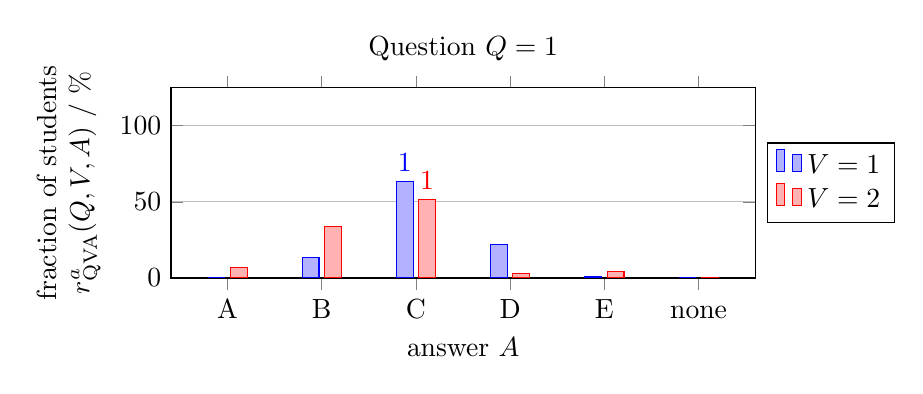
\begin{tikzpicture}[baseline]
\begin{axis}[
title={Question $Q = 1$},
ybar, ymin=0, ymax=100,
width=9cm, height=4cm,
xlabel={answer $A$},
ylabel={\parbox{9em}{\centering fraction of students \\ $r^a_{\rm QVA}(Q,V,A)$ / \%}},
symbolic x coords={A,B,C,D,E,none},
xticklabels={A,B,C,D,E,\vphantom{A}none},
xtick=data,
ymajorgrids=true,
enlarge x limits=0.12,
enlarge y limits={upper,value=0.25},
legend style={at={(1.02,0.5)},anchor=west},
bar width=0.214286cm,
point meta=explicit,
nodes near coords={\pgfmathfloatifflags{\pgfplotspointmeta}{0}{}{\pgfmathprintnumber{\pgfplotspointmeta}}},
]
\addplot coordinates {
(A,0) [0]
(B,13.41) [0]
(C,63.2184) [1]
(D,22.2222) [0]
(E,1.14943) [0]
(none,0) [0]
};
\addplot coordinates {
(A,6.86499) [0]
(B,33.8673) [0]
(C,51.7162) [1]
(D,2.97483) [0]
(E,4.11899) [0]
(none,0.457666) [0]
};
\legend{$V = 1$,$V = 2$};
\end{axis}
\end{tikzpicture}
\hfill
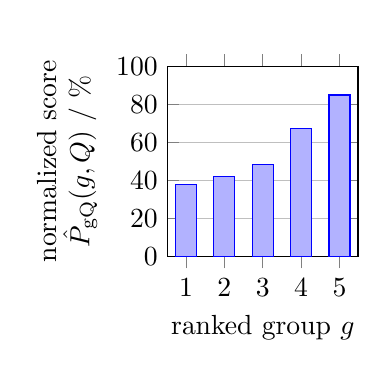
\begin{tikzpicture}[baseline]
\begin{axis}[
ybar, ymin=0, ymax=100,
xmin=1, xmax=5,
width=4cm, height=4cm,
symbolic x coords={1,2,3,4,5},
xtick=data,
xlabel={ranked group $g$},
ylabel={\parbox{9em}{\centering normalized score \\ $\hat{P}_{\rm gQ}(g,Q)$ / \%}},
ymajorgrids=true,
enlarge x limits=0.12,
bar width=0.266667cm,
]
\addplot coordinates {
(1,37.8571)
(2,42.1429)
(3,48.2014)
(4,67.1429)
(5,84.8921)
};
\end{axis}
\end{tikzpicture}

\end{minipage}

\vspace{1cm}
\noindent
\begin{minipage}{\textwidth}
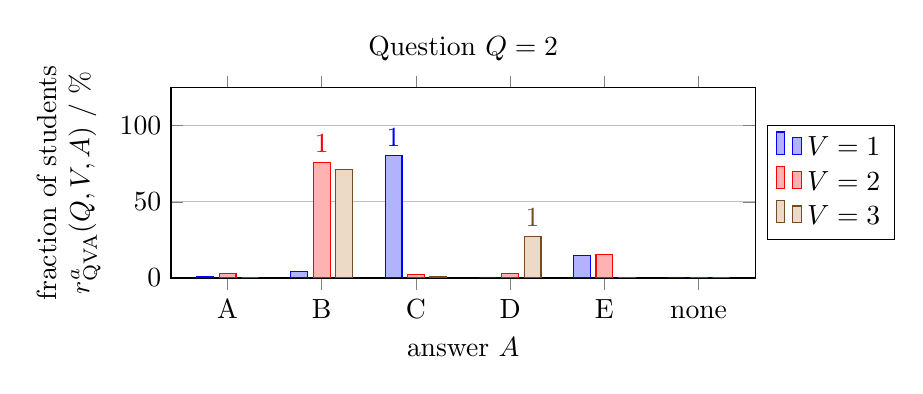
\begin{tikzpicture}[baseline]
\begin{axis}[
title={Question $Q = 2$},
ybar, ymin=0, ymax=100,
width=9cm, height=4cm,
xlabel={answer $A$},
ylabel={\parbox{9em}{\centering fraction of students \\ $r^a_{\rm QVA}(Q,V,A)$ / \%}},
symbolic x coords={A,B,C,D,E,none},
xticklabels={A,B,C,D,E,\vphantom{A}none},
xtick=data,
ymajorgrids=true,
enlarge x limits=0.12,
enlarge y limits={upper,value=0.25},
legend style={at={(1.02,0.5)},anchor=west},
bar width=0.214286cm,
point meta=explicit,
nodes near coords={\pgfmathfloatifflags{\pgfplotspointmeta}{0}{}{\pgfmathprintnumber{\pgfplotspointmeta}}},
]
\addplot coordinates {
(A,0.862069) [0]
(B,4.31034) [0]
(C,80.1724) [1]
(D,0) [0]
(E,14.6552) [0]
(none,0) [0]
};
\addplot coordinates {
(A,2.94118) [0]
(B,75.8824) [1]
(C,2.35294) [0]
(D,2.94118) [0]
(E,15.2941) [0]
(none,0.588235) [0]
};
\addplot coordinates {
(A,0) [0]
(B,71.2838) [0]
(C,1.01351) [0]
(D,27.3649) [1]
(E,0.337838) [0]
(none,0) [0]
};
\legend{$V = 1$,$V = 2$,$V = 3$};
\end{axis}
\end{tikzpicture}
\hfill
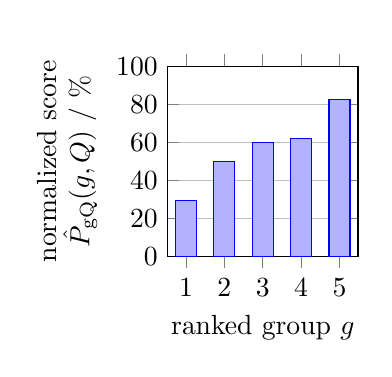
\begin{tikzpicture}[baseline]
\begin{axis}[
ybar, ymin=0, ymax=100,
xmin=1, xmax=5,
width=4cm, height=4cm,
symbolic x coords={1,2,3,4,5},
xtick=data,
xlabel={ranked group $g$},
ylabel={\parbox{9em}{\centering normalized score \\ $\hat{P}_{\rm gQ}(g,Q)$ / \%}},
ymajorgrids=true,
enlarge x limits=0.12,
bar width=0.266667cm,
]
\addplot coordinates {
(1,29.2857)
(2,50)
(3,59.7122)
(4,62.1429)
(5,82.7338)
};
\end{axis}
\end{tikzpicture}

\end{minipage}

\vspace{1cm}
\noindent
\begin{minipage}{\textwidth}
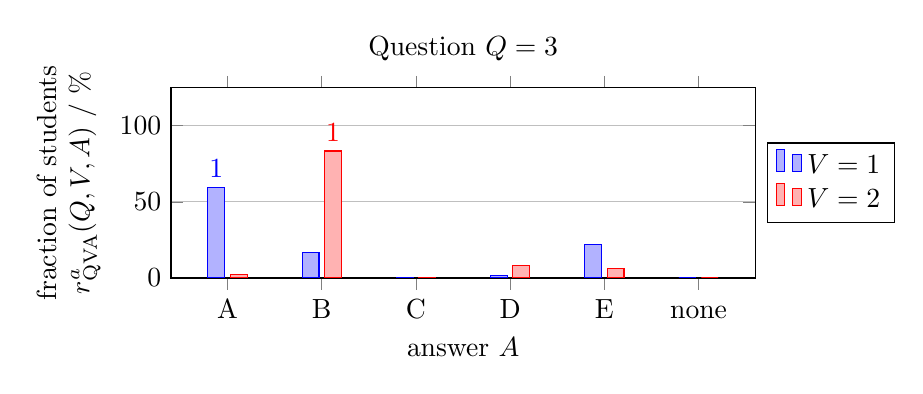
\begin{tikzpicture}[baseline]
\begin{axis}[
title={Question $Q = 3$},
ybar, ymin=0, ymax=100,
width=9cm, height=4cm,
xlabel={answer $A$},
ylabel={\parbox{9em}{\centering fraction of students \\ $r^a_{\rm QVA}(Q,V,A)$ / \%}},
symbolic x coords={A,B,C,D,E,none},
xticklabels={A,B,C,D,E,\vphantom{A}none},
xtick=data,
ymajorgrids=true,
enlarge x limits=0.12,
enlarge y limits={upper,value=0.25},
legend style={at={(1.02,0.5)},anchor=west},
bar width=0.214286cm,
point meta=explicit,
nodes near coords={\pgfmathfloatifflags{\pgfplotspointmeta}{0}{}{\pgfmathprintnumber{\pgfplotspointmeta}}},
]
\addplot coordinates {
(A,59.3846) [1]
(B,16.6154) [0]
(C,0.307692) [0]
(D,1.53846) [0]
(E,22.1538) [0]
(none,0) [0]
};
\addplot coordinates {
(A,2.14477) [0]
(B,83.378) [1]
(C,0.268097) [0]
(D,8.0429) [0]
(E,6.16622) [0]
(none,0) [0]
};
\legend{$V = 1$,$V = 2$};
\end{axis}
\end{tikzpicture}
\hfill
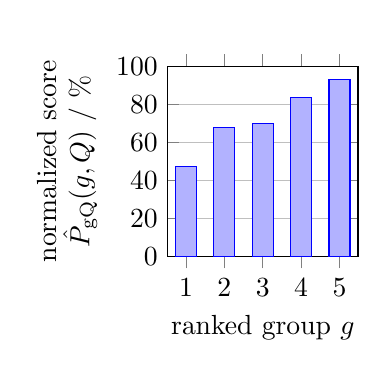
\begin{tikzpicture}[baseline]
\begin{axis}[
ybar, ymin=0, ymax=100,
xmin=1, xmax=5,
width=4cm, height=4cm,
symbolic x coords={1,2,3,4,5},
xtick=data,
xlabel={ranked group $g$},
ylabel={\parbox{9em}{\centering normalized score \\ $\hat{P}_{\rm gQ}(g,Q)$ / \%}},
ymajorgrids=true,
enlarge x limits=0.12,
bar width=0.266667cm,
]
\addplot coordinates {
(1,47.1429)
(2,67.8571)
(3,69.7842)
(4,83.5714)
(5,92.8058)
};
\end{axis}
\end{tikzpicture}

\end{minipage}

\vspace{1cm}
\noindent
\begin{minipage}{\textwidth}
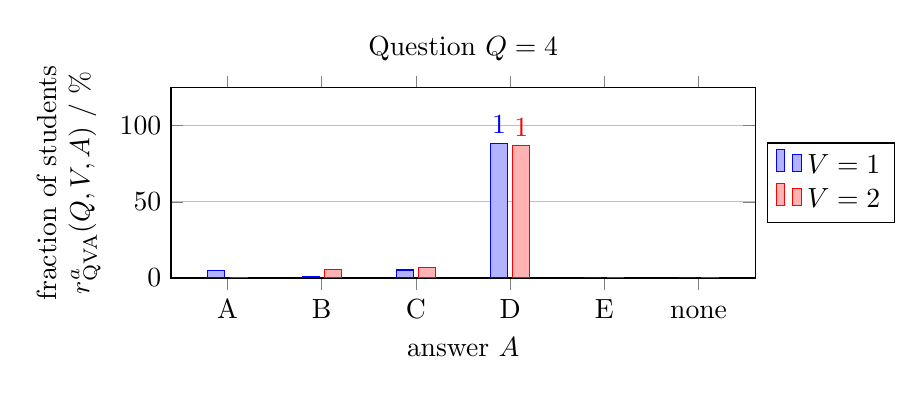
\begin{tikzpicture}[baseline]
\begin{axis}[
title={Question $Q = 4$},
ybar, ymin=0, ymax=100,
width=9cm, height=4cm,
xlabel={answer $A$},
ylabel={\parbox{9em}{\centering fraction of students \\ $r^a_{\rm QVA}(Q,V,A)$ / \%}},
symbolic x coords={A,B,C,D,E,none},
xticklabels={A,B,C,D,E,\vphantom{A}none},
xtick=data,
ymajorgrids=true,
enlarge x limits=0.12,
enlarge y limits={upper,value=0.25},
legend style={at={(1.02,0.5)},anchor=west},
bar width=0.214286cm,
point meta=explicit,
nodes near coords={\pgfmathfloatifflags{\pgfplotspointmeta}{0}{}{\pgfmathprintnumber{\pgfplotspointmeta}}},
]
\addplot coordinates {
(A,4.96894) [0]
(B,1.24224) [0]
(C,5.2795) [0]
(D,88.1988) [1]
(E,0) [0]
(none,0.310559) [0]
};
\addplot coordinates {
(A,0.531915) [0]
(B,5.58511) [0]
(C,6.91489) [0]
(D,86.7021) [1]
(E,0) [0]
(none,0.265957) [0]
};
\legend{$V = 1$,$V = 2$};
\end{axis}
\end{tikzpicture}
\hfill
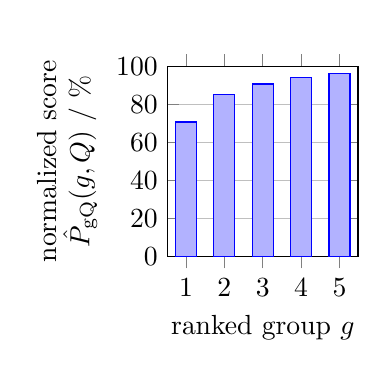
\begin{tikzpicture}[baseline]
\begin{axis}[
ybar, ymin=0, ymax=100,
xmin=1, xmax=5,
width=4cm, height=4cm,
symbolic x coords={1,2,3,4,5},
xtick=data,
xlabel={ranked group $g$},
ylabel={\parbox{9em}{\centering normalized score \\ $\hat{P}_{\rm gQ}(g,Q)$ / \%}},
ymajorgrids=true,
enlarge x limits=0.12,
bar width=0.266667cm,
]
\addplot coordinates {
(1,70.7143)
(2,85)
(3,90.6475)
(4,94.2857)
(5,96.4029)
};
\end{axis}
\end{tikzpicture}

\end{minipage}

\vspace{1cm}
\noindent
\begin{minipage}{\textwidth}
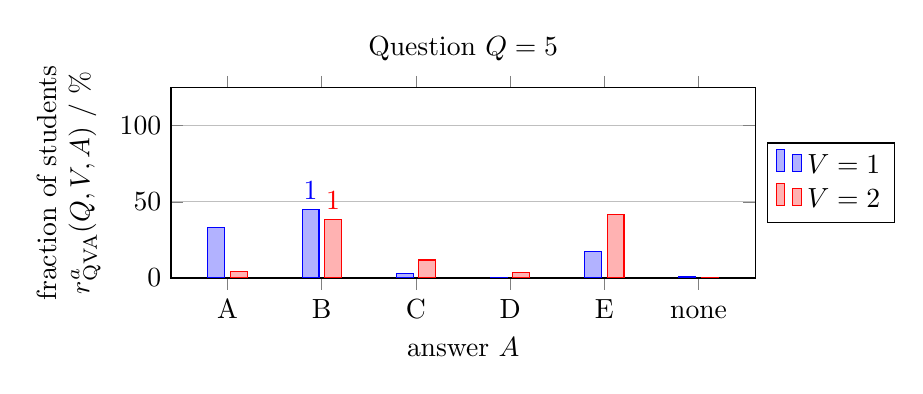
\begin{tikzpicture}[baseline]
\begin{axis}[
title={Question $Q = 5$},
ybar, ymin=0, ymax=100,
width=9cm, height=4cm,
xlabel={answer $A$},
ylabel={\parbox{9em}{\centering fraction of students \\ $r^a_{\rm QVA}(Q,V,A)$ / \%}},
symbolic x coords={A,B,C,D,E,none},
xticklabels={A,B,C,D,E,\vphantom{A}none},
xtick=data,
ymajorgrids=true,
enlarge x limits=0.12,
enlarge y limits={upper,value=0.25},
legend style={at={(1.02,0.5)},anchor=west},
bar width=0.214286cm,
point meta=explicit,
nodes near coords={\pgfmathfloatifflags{\pgfplotspointmeta}{0}{}{\pgfmathprintnumber{\pgfplotspointmeta}}},
]
\addplot coordinates {
(A,33.2425) [0]
(B,45.2316) [1]
(C,2.7248) [0]
(D,0.544959) [0]
(E,17.4387) [0]
(none,0.817439) [0]
};
\addplot coordinates {
(A,4.22961) [0]
(B,38.3686) [1]
(C,11.7825) [0]
(D,3.62538) [0]
(E,41.6918) [0]
(none,0.302115) [0]
};
\legend{$V = 1$,$V = 2$};
\end{axis}
\end{tikzpicture}
\hfill
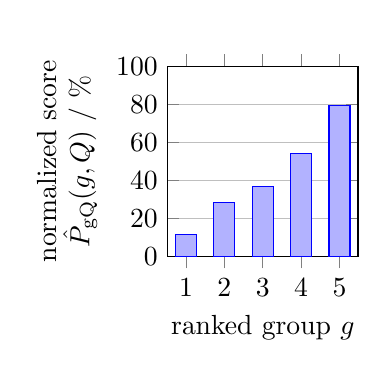
\begin{tikzpicture}[baseline]
\begin{axis}[
ybar, ymin=0, ymax=100,
xmin=1, xmax=5,
width=4cm, height=4cm,
symbolic x coords={1,2,3,4,5},
xtick=data,
xlabel={ranked group $g$},
ylabel={\parbox{9em}{\centering normalized score \\ $\hat{P}_{\rm gQ}(g,Q)$ / \%}},
ymajorgrids=true,
enlarge x limits=0.12,
bar width=0.266667cm,
]
\addplot coordinates {
(1,11.4286)
(2,28.5714)
(3,36.6906)
(4,54.2857)
(5,79.1367)
};
\end{axis}
\end{tikzpicture}

\end{minipage}

\vspace{1cm}
\noindent
\begin{minipage}{\textwidth}
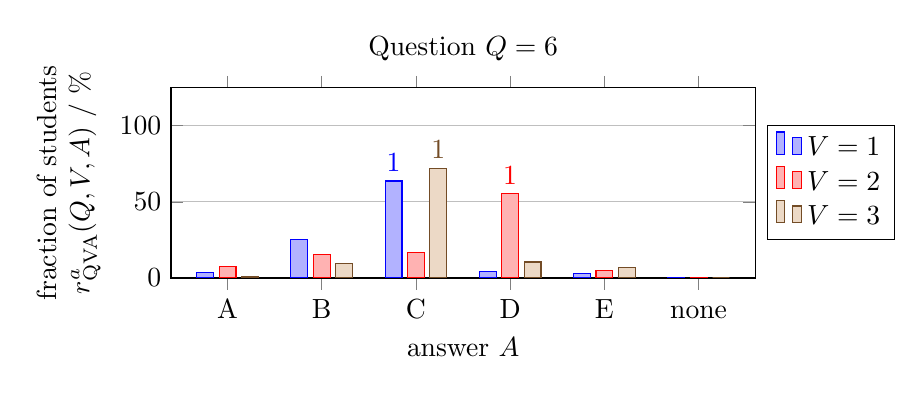
\begin{tikzpicture}[baseline]
\begin{axis}[
title={Question $Q = 6$},
ybar, ymin=0, ymax=100,
width=9cm, height=4cm,
xlabel={answer $A$},
ylabel={\parbox{9em}{\centering fraction of students \\ $r^a_{\rm QVA}(Q,V,A)$ / \%}},
symbolic x coords={A,B,C,D,E,none},
xticklabels={A,B,C,D,E,\vphantom{A}none},
xtick=data,
ymajorgrids=true,
enlarge x limits=0.12,
enlarge y limits={upper,value=0.25},
legend style={at={(1.02,0.5)},anchor=west},
bar width=0.214286cm,
point meta=explicit,
nodes near coords={\pgfmathfloatifflags{\pgfplotspointmeta}{0}{}{\pgfmathprintnumber{\pgfplotspointmeta}}},
]
\addplot coordinates {
(A,3.40909) [0]
(B,25) [0]
(C,63.6364) [1]
(D,4.54545) [0]
(E,2.84091) [0]
(none,0.568182) [0]
};
\addplot coordinates {
(A,7.27273) [0]
(B,15.6364) [0]
(C,16.7273) [0]
(D,55.2727) [1]
(E,4.72727) [0]
(none,0.363636) [0]
};
\addplot coordinates {
(A,0.809717) [0]
(B,9.7166) [0]
(C,72.0648) [1]
(D,10.5263) [0]
(E,6.88259) [0]
(none,0) [0]
};
\legend{$V = 1$,$V = 2$,$V = 3$};
\end{axis}
\end{tikzpicture}
\hfill
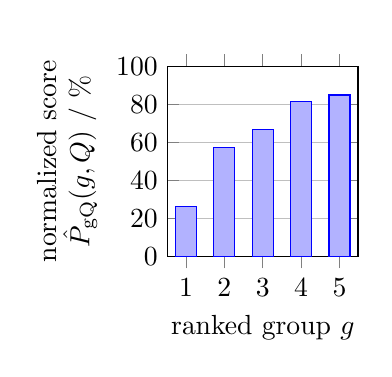
\begin{tikzpicture}[baseline]
\begin{axis}[
ybar, ymin=0, ymax=100,
xmin=1, xmax=5,
width=4cm, height=4cm,
symbolic x coords={1,2,3,4,5},
xtick=data,
xlabel={ranked group $g$},
ylabel={\parbox{9em}{\centering normalized score \\ $\hat{P}_{\rm gQ}(g,Q)$ / \%}},
ymajorgrids=true,
enlarge x limits=0.12,
bar width=0.266667cm,
]
\addplot coordinates {
(1,26.4286)
(2,57.1429)
(3,66.9065)
(4,81.4286)
(5,84.8921)
};
\end{axis}
\end{tikzpicture}

\end{minipage}

\vspace{1cm}
\noindent
\begin{minipage}{\textwidth}
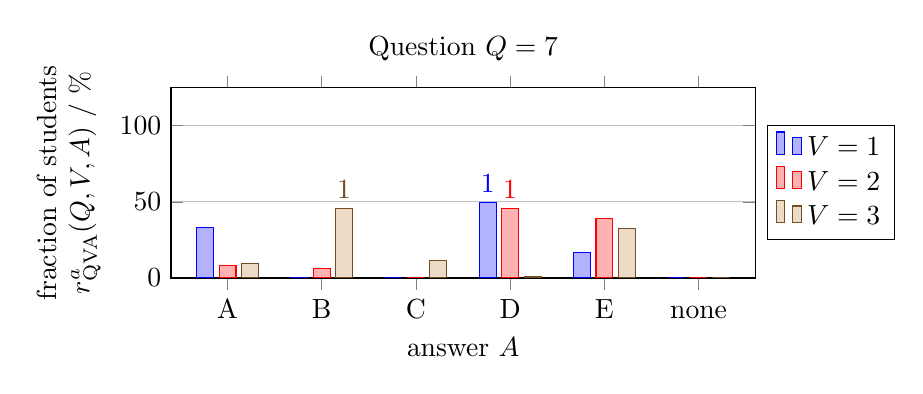
\begin{tikzpicture}[baseline]
\begin{axis}[
title={Question $Q = 7$},
ybar, ymin=0, ymax=100,
width=9cm, height=4cm,
xlabel={answer $A$},
ylabel={\parbox{9em}{\centering fraction of students \\ $r^a_{\rm QVA}(Q,V,A)$ / \%}},
symbolic x coords={A,B,C,D,E,none},
xticklabels={A,B,C,D,E,\vphantom{A}none},
xtick=data,
ymajorgrids=true,
enlarge x limits=0.12,
enlarge y limits={upper,value=0.25},
legend style={at={(1.02,0.5)},anchor=west},
bar width=0.214286cm,
point meta=explicit,
nodes near coords={\pgfmathfloatifflags{\pgfplotspointmeta}{0}{}{\pgfmathprintnumber{\pgfplotspointmeta}}},
]
\addplot coordinates {
(A,33.3333) [0]
(B,0.392157) [0]
(C,0) [0]
(D,49.4118) [1]
(E,16.8627) [0]
(none,0) [0]
};
\addplot coordinates {
(A,8.45771) [0]
(B,6.46766) [0]
(C,0) [0]
(D,45.7711) [1]
(E,39.3035) [0]
(none,0) [0]
};
\addplot coordinates {
(A,9.50413) [0]
(B,45.4545) [1]
(C,11.5702) [0]
(D,0.826446) [0]
(E,32.6446) [0]
(none,0) [0]
};
\legend{$V = 1$,$V = 2$,$V = 3$};
\end{axis}
\end{tikzpicture}
\hfill
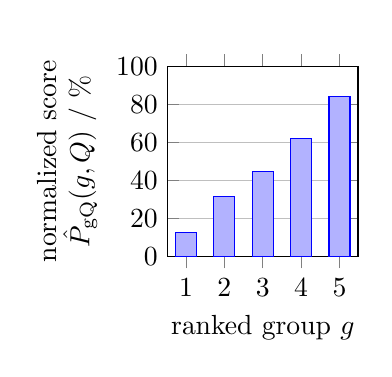
\begin{tikzpicture}[baseline]
\begin{axis}[
ybar, ymin=0, ymax=100,
xmin=1, xmax=5,
width=4cm, height=4cm,
symbolic x coords={1,2,3,4,5},
xtick=data,
xlabel={ranked group $g$},
ylabel={\parbox{9em}{\centering normalized score \\ $\hat{P}_{\rm gQ}(g,Q)$ / \%}},
ymajorgrids=true,
enlarge x limits=0.12,
bar width=0.266667cm,
]
\addplot coordinates {
(1,12.8571)
(2,31.4286)
(3,44.6043)
(4,62.1429)
(5,84.1727)
};
\end{axis}
\end{tikzpicture}

\end{minipage}

\vspace{1cm}
\noindent
\begin{minipage}{\textwidth}
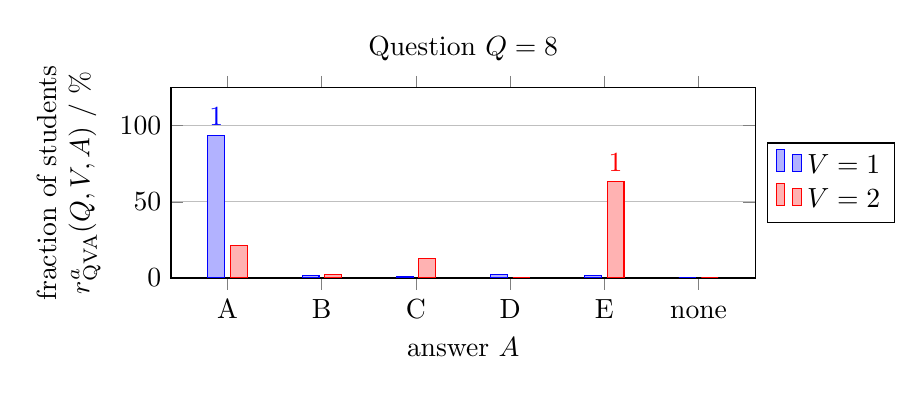
\begin{tikzpicture}[baseline]
\begin{axis}[
title={Question $Q = 8$},
ybar, ymin=0, ymax=100,
width=9cm, height=4cm,
xlabel={answer $A$},
ylabel={\parbox{9em}{\centering fraction of students \\ $r^a_{\rm QVA}(Q,V,A)$ / \%}},
symbolic x coords={A,B,C,D,E,none},
xticklabels={A,B,C,D,E,\vphantom{A}none},
xtick=data,
ymajorgrids=true,
enlarge x limits=0.12,
enlarge y limits={upper,value=0.25},
legend style={at={(1.02,0.5)},anchor=west},
bar width=0.214286cm,
point meta=explicit,
nodes near coords={\pgfmathfloatifflags{\pgfplotspointmeta}{0}{}{\pgfmathprintnumber{\pgfplotspointmeta}}},
]
\addplot coordinates {
(A,93.379) [1]
(B,1.82648) [0]
(C,0.913242) [0]
(D,2.05479) [0]
(E,1.82648) [0]
(none,0) [0]
};
\addplot coordinates {
(A,21.5385) [0]
(B,2.30769) [0]
(C,12.6923) [0]
(D,0) [0]
(E,63.4615) [1]
(none,0) [0]
};
\legend{$V = 1$,$V = 2$};
\end{axis}
\end{tikzpicture}
\hfill
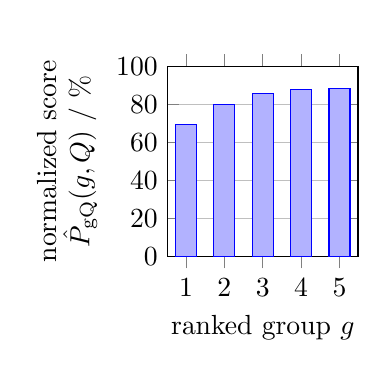
\begin{tikzpicture}[baseline]
\begin{axis}[
ybar, ymin=0, ymax=100,
xmin=1, xmax=5,
width=4cm, height=4cm,
symbolic x coords={1,2,3,4,5},
xtick=data,
xlabel={ranked group $g$},
ylabel={\parbox{9em}{\centering normalized score \\ $\hat{P}_{\rm gQ}(g,Q)$ / \%}},
ymajorgrids=true,
enlarge x limits=0.12,
bar width=0.266667cm,
]
\addplot coordinates {
(1,69.2857)
(2,80)
(3,85.6115)
(4,87.8571)
(5,88.4892)
};
\end{axis}
\end{tikzpicture}

\end{minipage}

\vspace{1cm}
\noindent
\begin{minipage}{\textwidth}
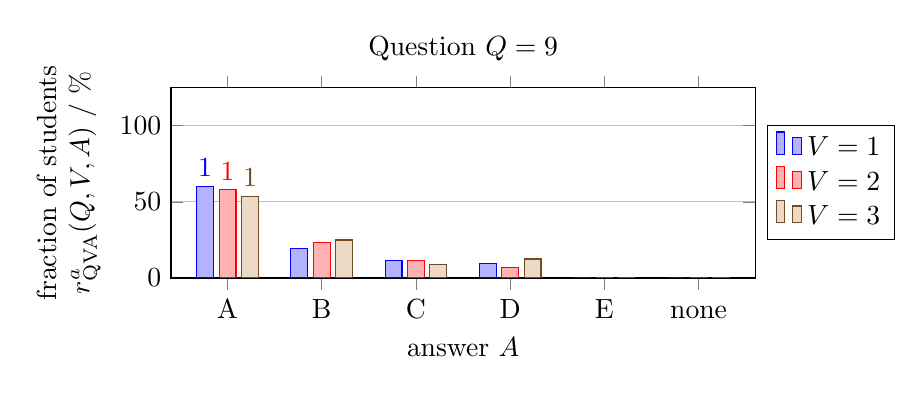
\begin{tikzpicture}[baseline]
\begin{axis}[
title={Question $Q = 9$},
ybar, ymin=0, ymax=100,
width=9cm, height=4cm,
xlabel={answer $A$},
ylabel={\parbox{9em}{\centering fraction of students \\ $r^a_{\rm QVA}(Q,V,A)$ / \%}},
symbolic x coords={A,B,C,D,E,none},
xticklabels={A,B,C,D,E,\vphantom{A}none},
xtick=data,
ymajorgrids=true,
enlarge x limits=0.12,
enlarge y limits={upper,value=0.25},
legend style={at={(1.02,0.5)},anchor=west},
bar width=0.214286cm,
point meta=explicit,
nodes near coords={\pgfmathfloatifflags{\pgfplotspointmeta}{0}{}{\pgfmathprintnumber{\pgfplotspointmeta}}},
]
\addplot coordinates {
(A,60) [1]
(B,19.3333) [0]
(C,11.3333) [0]
(D,9.33333) [0]
(E,0) [0]
(none,0) [0]
};
\addplot coordinates {
(A,57.8199) [1]
(B,23.2227) [0]
(C,11.3744) [0]
(D,7.109) [0]
(E,0) [0]
(none,0.473934) [0]
};
\addplot coordinates {
(A,53.4125) [1]
(B,24.9258) [0]
(C,8.90208) [0]
(D,12.4629) [0]
(E,0) [0]
(none,0.296736) [0]
};
\legend{$V = 1$,$V = 2$,$V = 3$};
\end{axis}
\end{tikzpicture}
\hfill
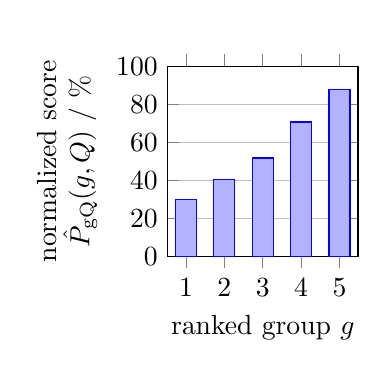
\begin{tikzpicture}[baseline]
\begin{axis}[
ybar, ymin=0, ymax=100,
xmin=1, xmax=5,
width=4cm, height=4cm,
symbolic x coords={1,2,3,4,5},
xtick=data,
xlabel={ranked group $g$},
ylabel={\parbox{9em}{\centering normalized score \\ $\hat{P}_{\rm gQ}(g,Q)$ / \%}},
ymajorgrids=true,
enlarge x limits=0.12,
bar width=0.266667cm,
]
\addplot coordinates {
(1,30)
(2,40.7143)
(3,51.7986)
(4,70.7143)
(5,87.7698)
};
\end{axis}
\end{tikzpicture}

\end{minipage}

\vspace{1cm}
\noindent
\begin{minipage}{\textwidth}
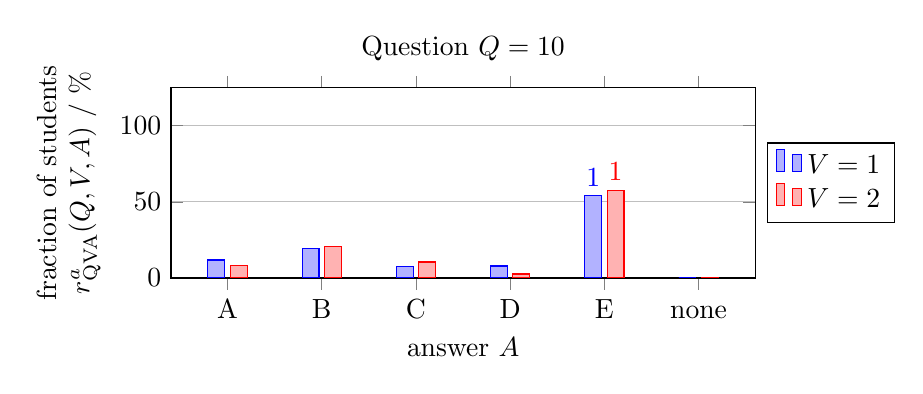
\begin{tikzpicture}[baseline]
\begin{axis}[
title={Question $Q = 10$},
ybar, ymin=0, ymax=100,
width=9cm, height=4cm,
xlabel={answer $A$},
ylabel={\parbox{9em}{\centering fraction of students \\ $r^a_{\rm QVA}(Q,V,A)$ / \%}},
symbolic x coords={A,B,C,D,E,none},
xticklabels={A,B,C,D,E,\vphantom{A}none},
xtick=data,
ymajorgrids=true,
enlarge x limits=0.12,
enlarge y limits={upper,value=0.25},
legend style={at={(1.02,0.5)},anchor=west},
bar width=0.214286cm,
point meta=explicit,
nodes near coords={\pgfmathfloatifflags{\pgfplotspointmeta}{0}{}{\pgfmathprintnumber{\pgfplotspointmeta}}},
]
\addplot coordinates {
(A,11.7978) [0]
(B,19.1011) [0]
(C,7.30337) [0]
(D,7.86517) [0]
(E,53.9326) [1]
(none,0) [0]
};
\addplot coordinates {
(A,8.18713) [0]
(B,20.7602) [0]
(C,10.5263) [0]
(D,2.63158) [0]
(E,57.6023) [1]
(none,0.292398) [0]
};
\legend{$V = 1$,$V = 2$};
\end{axis}
\end{tikzpicture}
\hfill
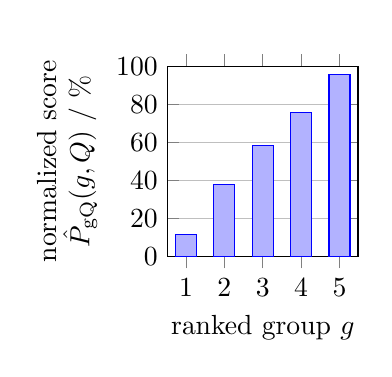
\begin{tikzpicture}[baseline]
\begin{axis}[
ybar, ymin=0, ymax=100,
xmin=1, xmax=5,
width=4cm, height=4cm,
symbolic x coords={1,2,3,4,5},
xtick=data,
xlabel={ranked group $g$},
ylabel={\parbox{9em}{\centering normalized score \\ $\hat{P}_{\rm gQ}(g,Q)$ / \%}},
ymajorgrids=true,
enlarge x limits=0.12,
bar width=0.266667cm,
]
\addplot coordinates {
(1,11.4286)
(2,37.8571)
(3,58.2734)
(4,75.7143)
(5,95.6835)
};
\end{axis}
\end{tikzpicture}

\end{minipage}

\vspace{1cm}
\noindent
\begin{minipage}{\textwidth}
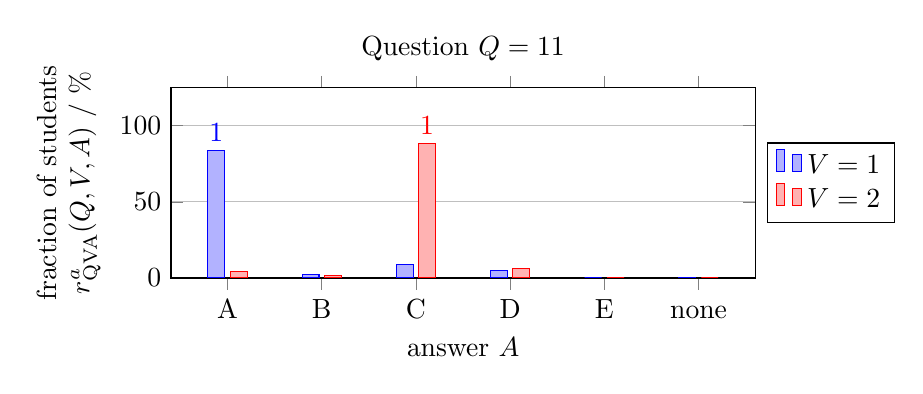
\begin{tikzpicture}[baseline]
\begin{axis}[
title={Question $Q = 11$},
ybar, ymin=0, ymax=100,
width=9cm, height=4cm,
xlabel={answer $A$},
ylabel={\parbox{9em}{\centering fraction of students \\ $r^a_{\rm QVA}(Q,V,A)$ / \%}},
symbolic x coords={A,B,C,D,E,none},
xticklabels={A,B,C,D,E,\vphantom{A}none},
xtick=data,
ymajorgrids=true,
enlarge x limits=0.12,
enlarge y limits={upper,value=0.25},
legend style={at={(1.02,0.5)},anchor=west},
bar width=0.214286cm,
point meta=explicit,
nodes near coords={\pgfmathfloatifflags{\pgfplotspointmeta}{0}{}{\pgfmathprintnumber{\pgfplotspointmeta}}},
]
\addplot coordinates {
(A,83.4452) [1]
(B,2.23714) [0]
(C,8.94855) [0]
(D,4.9217) [0]
(E,0) [0]
(none,0.447427) [0]
};
\addplot coordinates {
(A,3.98406) [0]
(B,1.59363) [0]
(C,88.0478) [1]
(D,6.3745) [0]
(E,0) [0]
(none,0) [0]
};
\legend{$V = 1$,$V = 2$};
\end{axis}
\end{tikzpicture}
\hfill
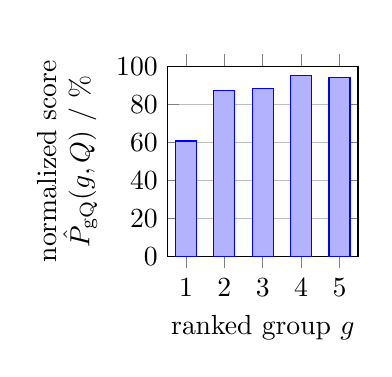
\begin{tikzpicture}[baseline]
\begin{axis}[
ybar, ymin=0, ymax=100,
xmin=1, xmax=5,
width=4cm, height=4cm,
symbolic x coords={1,2,3,4,5},
xtick=data,
xlabel={ranked group $g$},
ylabel={\parbox{9em}{\centering normalized score \\ $\hat{P}_{\rm gQ}(g,Q)$ / \%}},
ymajorgrids=true,
enlarge x limits=0.12,
bar width=0.266667cm,
]
\addplot coordinates {
(1,60.7143)
(2,87.1429)
(3,88.4892)
(4,95)
(5,94.2446)
};
\end{axis}
\end{tikzpicture}

\end{minipage}

\vspace{1cm}
\noindent
\begin{minipage}{\textwidth}
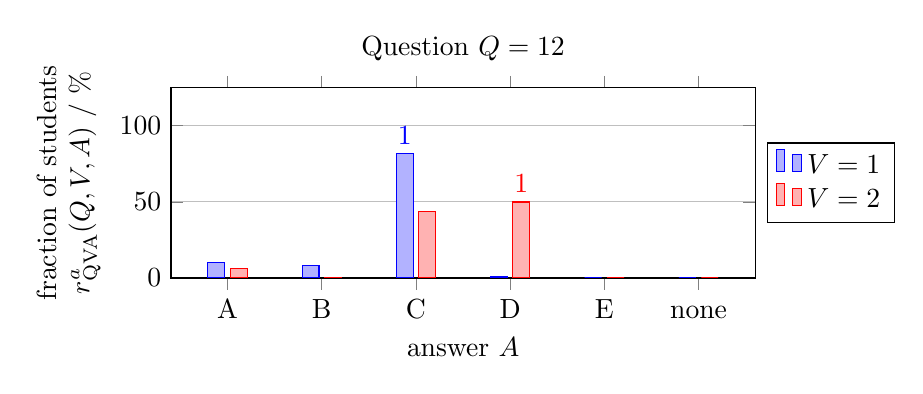
\begin{tikzpicture}[baseline]
\begin{axis}[
title={Question $Q = 12$},
ybar, ymin=0, ymax=100,
width=9cm, height=4cm,
xlabel={answer $A$},
ylabel={\parbox{9em}{\centering fraction of students \\ $r^a_{\rm QVA}(Q,V,A)$ / \%}},
symbolic x coords={A,B,C,D,E,none},
xticklabels={A,B,C,D,E,\vphantom{A}none},
xtick=data,
ymajorgrids=true,
enlarge x limits=0.12,
enlarge y limits={upper,value=0.25},
legend style={at={(1.02,0.5)},anchor=west},
bar width=0.214286cm,
point meta=explicit,
nodes near coords={\pgfmathfloatifflags{\pgfplotspointmeta}{0}{}{\pgfmathprintnumber{\pgfplotspointmeta}}},
]
\addplot coordinates {
(A,9.90415) [0]
(B,7.98722) [0]
(C,81.4696) [1]
(D,0.638978) [0]
(E,0) [0]
(none,0) [0]
};
\addplot coordinates {
(A,6.23377) [0]
(B,0.25974) [0]
(C,43.6364) [0]
(D,49.8701) [1]
(E,0) [0]
(none,0) [0]
};
\legend{$V = 1$,$V = 2$};
\end{axis}
\end{tikzpicture}
\hfill
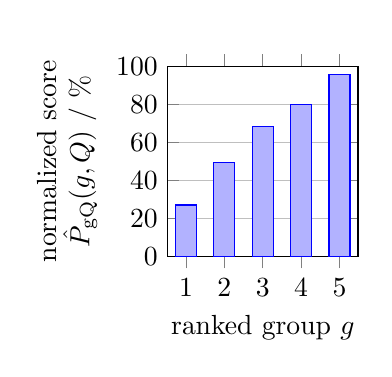
\begin{tikzpicture}[baseline]
\begin{axis}[
ybar, ymin=0, ymax=100,
xmin=1, xmax=5,
width=4cm, height=4cm,
symbolic x coords={1,2,3,4,5},
xtick=data,
xlabel={ranked group $g$},
ylabel={\parbox{9em}{\centering normalized score \\ $\hat{P}_{\rm gQ}(g,Q)$ / \%}},
ymajorgrids=true,
enlarge x limits=0.12,
bar width=0.266667cm,
]
\addplot coordinates {
(1,27.1429)
(2,49.2857)
(3,68.3453)
(4,80)
(5,95.6835)
};
\end{axis}
\end{tikzpicture}

\end{minipage}

\vspace{1cm}
\noindent
\begin{minipage}{\textwidth}
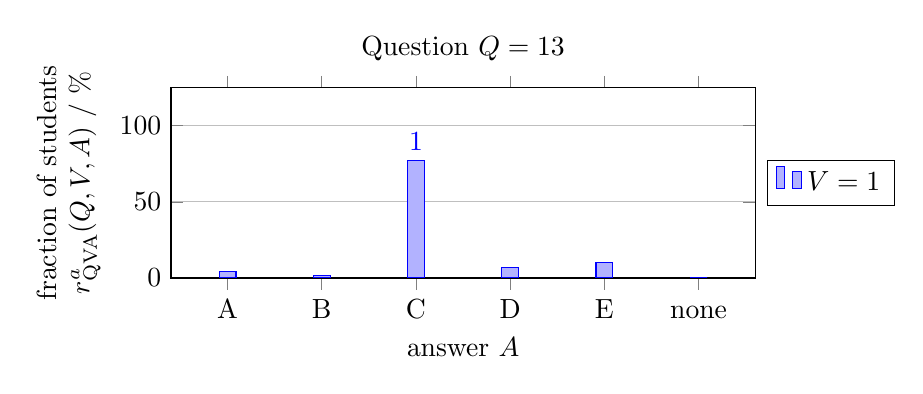
\begin{tikzpicture}[baseline]
\begin{axis}[
title={Question $Q = 13$},
ybar, ymin=0, ymax=100,
width=9cm, height=4cm,
xlabel={answer $A$},
ylabel={\parbox{9em}{\centering fraction of students \\ $r^a_{\rm QVA}(Q,V,A)$ / \%}},
symbolic x coords={A,B,C,D,E,none},
xticklabels={A,B,C,D,E,\vphantom{A}none},
xtick=data,
ymajorgrids=true,
enlarge x limits=0.12,
enlarge y limits={upper,value=0.25},
legend style={at={(1.02,0.5)},anchor=west},
bar width=0.214286cm,
point meta=explicit,
nodes near coords={\pgfmathfloatifflags{\pgfplotspointmeta}{0}{}{\pgfmathprintnumber{\pgfplotspointmeta}}},
]
\addplot coordinates {
(A,4.15473) [0]
(B,1.86246) [0]
(C,77.0774) [1]
(D,6.73352) [0]
(E,10.1719) [0]
(none,0) [0]
};
\legend{$V = 1$};
\end{axis}
\end{tikzpicture}
\hfill
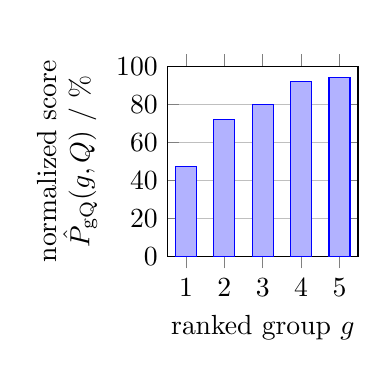
\begin{tikzpicture}[baseline]
\begin{axis}[
ybar, ymin=0, ymax=100,
xmin=1, xmax=5,
width=4cm, height=4cm,
symbolic x coords={1,2,3,4,5},
xtick=data,
xlabel={ranked group $g$},
ylabel={\parbox{9em}{\centering normalized score \\ $\hat{P}_{\rm gQ}(g,Q)$ / \%}},
ymajorgrids=true,
enlarge x limits=0.12,
bar width=0.266667cm,
]
\addplot coordinates {
(1,47.1429)
(2,72.1429)
(3,79.8561)
(4,92.1429)
(5,94.2446)
};
\end{axis}
\end{tikzpicture}

\end{minipage}

\vspace{1cm}
\noindent
\begin{minipage}{\textwidth}
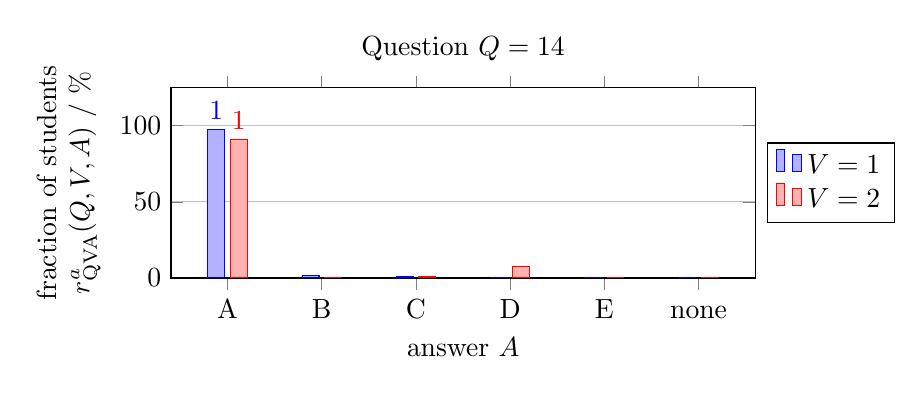
\begin{tikzpicture}[baseline]
\begin{axis}[
title={Question $Q = 14$},
ybar, ymin=0, ymax=100,
width=9cm, height=4cm,
xlabel={answer $A$},
ylabel={\parbox{9em}{\centering fraction of students \\ $r^a_{\rm QVA}(Q,V,A)$ / \%}},
symbolic x coords={A,B,C,D,E,none},
xticklabels={A,B,C,D,E,\vphantom{A}none},
xtick=data,
ymajorgrids=true,
enlarge x limits=0.12,
enlarge y limits={upper,value=0.25},
legend style={at={(1.02,0.5)},anchor=west},
bar width=0.214286cm,
point meta=explicit,
nodes near coords={\pgfmathfloatifflags{\pgfplotspointmeta}{0}{}{\pgfmathprintnumber{\pgfplotspointmeta}}},
]
\addplot coordinates {
(A,97.4638) [1]
(B,1.44928) [0]
(C,0.724638) [0]
(D,0.362319) [0]
(E,0) [0]
(none,0) [0]
};
\addplot coordinates {
(A,90.7583) [1]
(B,0.473934) [0]
(C,0.7109) [0]
(D,7.58294) [0]
(E,0) [0]
(none,0.473934) [0]
};
\legend{$V = 1$,$V = 2$};
\end{axis}
\end{tikzpicture}
\hfill
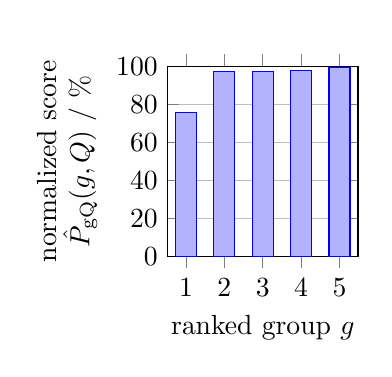
\begin{tikzpicture}[baseline]
\begin{axis}[
ybar, ymin=0, ymax=100,
xmin=1, xmax=5,
width=4cm, height=4cm,
symbolic x coords={1,2,3,4,5},
xtick=data,
xlabel={ranked group $g$},
ylabel={\parbox{9em}{\centering normalized score \\ $\hat{P}_{\rm gQ}(g,Q)$ / \%}},
ymajorgrids=true,
enlarge x limits=0.12,
bar width=0.266667cm,
]
\addplot coordinates {
(1,75.7143)
(2,97.1429)
(3,97.1223)
(4,97.8571)
(5,99.2806)
};
\end{axis}
\end{tikzpicture}

\end{minipage}

\vspace{1cm}
\noindent
\begin{minipage}{\textwidth}
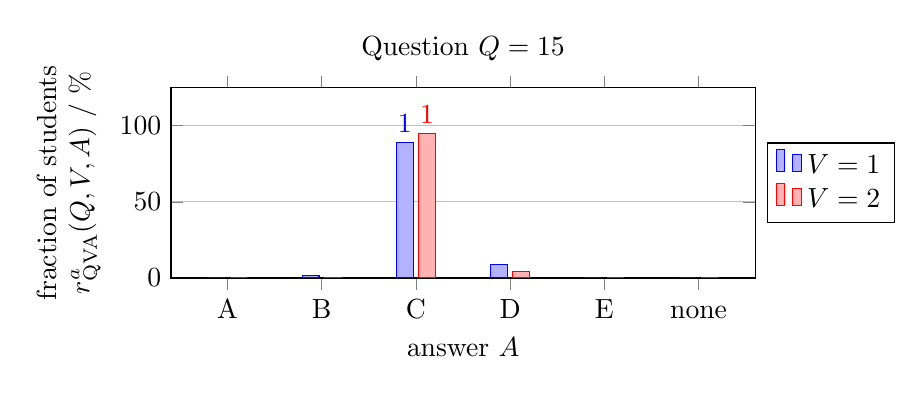
\begin{tikzpicture}[baseline]
\begin{axis}[
title={Question $Q = 15$},
ybar, ymin=0, ymax=100,
width=9cm, height=4cm,
xlabel={answer $A$},
ylabel={\parbox{9em}{\centering fraction of students \\ $r^a_{\rm QVA}(Q,V,A)$ / \%}},
symbolic x coords={A,B,C,D,E,none},
xticklabels={A,B,C,D,E,\vphantom{A}none},
xtick=data,
ymajorgrids=true,
enlarge x limits=0.12,
enlarge y limits={upper,value=0.25},
legend style={at={(1.02,0.5)},anchor=west},
bar width=0.214286cm,
point meta=explicit,
nodes near coords={\pgfmathfloatifflags{\pgfplotspointmeta}{0}{}{\pgfmathprintnumber{\pgfplotspointmeta}}},
]
\addplot coordinates {
(A,0.568182) [0]
(B,1.70455) [0]
(C,88.9205) [1]
(D,8.80682) [0]
(E,0) [0]
(none,0) [0]
};
\addplot coordinates {
(A,0) [0]
(B,0.578035) [0]
(C,95.0867) [1]
(D,4.33526) [0]
(E,0) [0]
(none,0) [0]
};
\legend{$V = 1$,$V = 2$};
\end{axis}
\end{tikzpicture}
\hfill
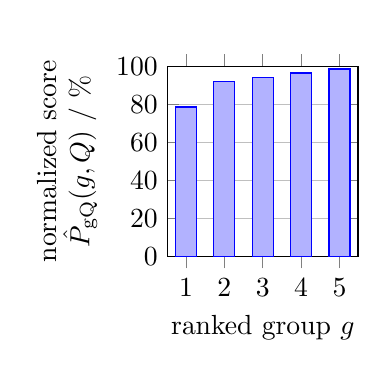
\begin{tikzpicture}[baseline]
\begin{axis}[
ybar, ymin=0, ymax=100,
xmin=1, xmax=5,
width=4cm, height=4cm,
symbolic x coords={1,2,3,4,5},
xtick=data,
xlabel={ranked group $g$},
ylabel={\parbox{9em}{\centering normalized score \\ $\hat{P}_{\rm gQ}(g,Q)$ / \%}},
ymajorgrids=true,
enlarge x limits=0.12,
bar width=0.266667cm,
]
\addplot coordinates {
(1,78.5714)
(2,92.1429)
(3,94.2446)
(4,96.4286)
(5,98.5612)
};
\end{axis}
\end{tikzpicture}

\end{minipage}

\vspace{1cm}
\noindent
\begin{minipage}{\textwidth}
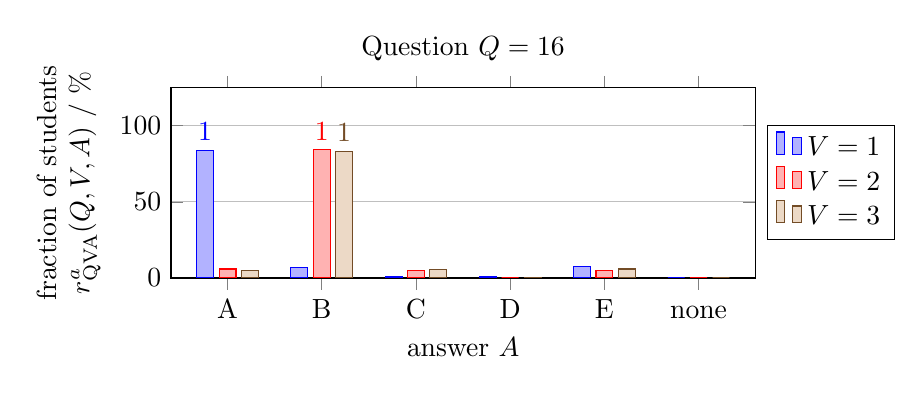
\begin{tikzpicture}[baseline]
\begin{axis}[
title={Question $Q = 16$},
ybar, ymin=0, ymax=100,
width=9cm, height=4cm,
xlabel={answer $A$},
ylabel={\parbox{9em}{\centering fraction of students \\ $r^a_{\rm QVA}(Q,V,A)$ / \%}},
symbolic x coords={A,B,C,D,E,none},
xticklabels={A,B,C,D,E,\vphantom{A}none},
xtick=data,
ymajorgrids=true,
enlarge x limits=0.12,
enlarge y limits={upper,value=0.25},
legend style={at={(1.02,0.5)},anchor=west},
bar width=0.214286cm,
point meta=explicit,
nodes near coords={\pgfmathfloatifflags{\pgfplotspointmeta}{0}{}{\pgfmathprintnumber{\pgfplotspointmeta}}},
]
\addplot coordinates {
(A,83.9806) [1]
(B,6.79612) [0]
(C,0.970874) [0]
(D,0.970874) [0]
(E,7.28155) [0]
(none,0) [0]
};
\addplot coordinates {
(A,5.90909) [0]
(B,84.0909) [1]
(C,5) [0]
(D,0) [0]
(E,5) [0]
(none,0) [0]
};
\addplot coordinates {
(A,5.14706) [0]
(B,83.0882) [1]
(C,5.51471) [0]
(D,0.367647) [0]
(E,5.88235) [0]
(none,0) [0]
};
\legend{$V = 1$,$V = 2$,$V = 3$};
\end{axis}
\end{tikzpicture}
\hfill
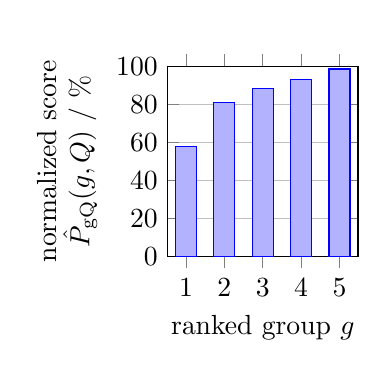
\begin{tikzpicture}[baseline]
\begin{axis}[
ybar, ymin=0, ymax=100,
xmin=1, xmax=5,
width=4cm, height=4cm,
symbolic x coords={1,2,3,4,5},
xtick=data,
xlabel={ranked group $g$},
ylabel={\parbox{9em}{\centering normalized score \\ $\hat{P}_{\rm gQ}(g,Q)$ / \%}},
ymajorgrids=true,
enlarge x limits=0.12,
bar width=0.266667cm,
]
\addplot coordinates {
(1,57.8571)
(2,80.7143)
(3,88.4892)
(4,92.8571)
(5,98.5612)
};
\end{axis}
\end{tikzpicture}

\end{minipage}

\vspace{1cm}
\noindent
\begin{minipage}{\textwidth}
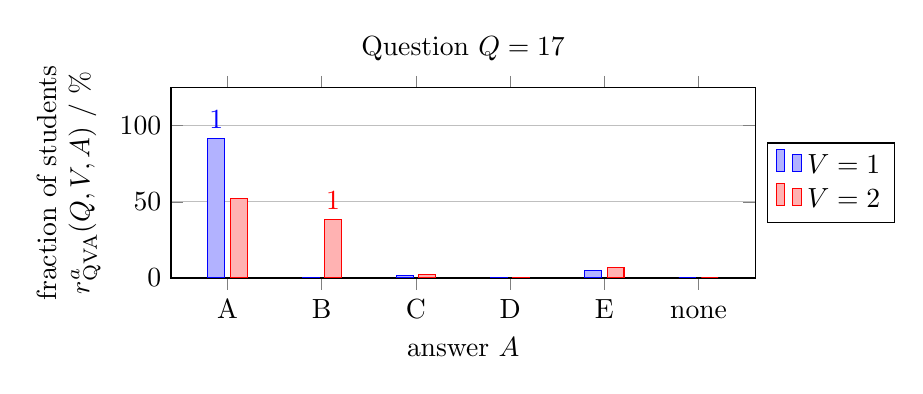
\begin{tikzpicture}[baseline]
\begin{axis}[
title={Question $Q = 17$},
ybar, ymin=0, ymax=100,
width=9cm, height=4cm,
xlabel={answer $A$},
ylabel={\parbox{9em}{\centering fraction of students \\ $r^a_{\rm QVA}(Q,V,A)$ / \%}},
symbolic x coords={A,B,C,D,E,none},
xticklabels={A,B,C,D,E,\vphantom{A}none},
xtick=data,
ymajorgrids=true,
enlarge x limits=0.12,
enlarge y limits={upper,value=0.25},
legend style={at={(1.02,0.5)},anchor=west},
bar width=0.214286cm,
point meta=explicit,
nodes near coords={\pgfmathfloatifflags{\pgfplotspointmeta}{0}{}{\pgfmathprintnumber{\pgfplotspointmeta}}},
]
\addplot coordinates {
(A,91.8033) [1]
(B,0.546448) [0]
(C,1.91257) [0]
(D,0.546448) [0]
(E,5.19126) [0]
(none,0) [0]
};
\addplot coordinates {
(A,52.1084) [0]
(B,38.5542) [1]
(C,2.40964) [0]
(D,0.301205) [0]
(E,6.62651) [0]
(none,0) [0]
};
\legend{$V = 1$,$V = 2$};
\end{axis}
\end{tikzpicture}
\hfill
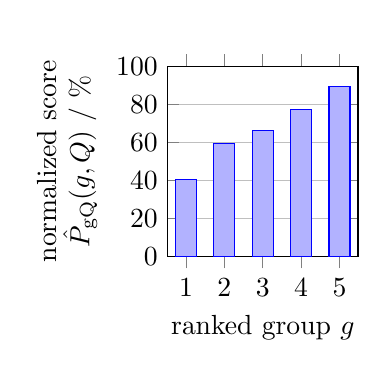
\begin{tikzpicture}[baseline]
\begin{axis}[
ybar, ymin=0, ymax=100,
xmin=1, xmax=5,
width=4cm, height=4cm,
symbolic x coords={1,2,3,4,5},
xtick=data,
xlabel={ranked group $g$},
ylabel={\parbox{9em}{\centering normalized score \\ $\hat{P}_{\rm gQ}(g,Q)$ / \%}},
ymajorgrids=true,
enlarge x limits=0.12,
bar width=0.266667cm,
]
\addplot coordinates {
(1,40.7143)
(2,59.2857)
(3,66.1871)
(4,77.1429)
(5,89.2086)
};
\end{axis}
\end{tikzpicture}

\end{minipage}

\vspace{1cm}
\noindent
\begin{minipage}{\textwidth}
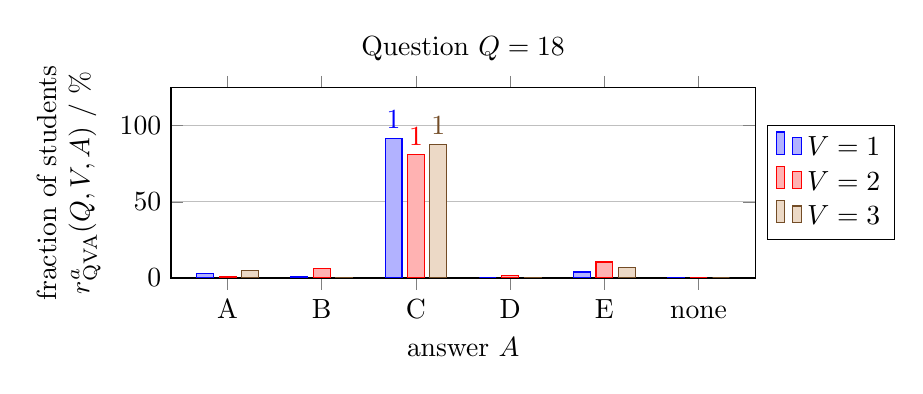
\begin{tikzpicture}[baseline]
\begin{axis}[
title={Question $Q = 18$},
ybar, ymin=0, ymax=100,
width=9cm, height=4cm,
xlabel={answer $A$},
ylabel={\parbox{9em}{\centering fraction of students \\ $r^a_{\rm QVA}(Q,V,A)$ / \%}},
symbolic x coords={A,B,C,D,E,none},
xticklabels={A,B,C,D,E,\vphantom{A}none},
xtick=data,
ymajorgrids=true,
enlarge x limits=0.12,
enlarge y limits={upper,value=0.25},
legend style={at={(1.02,0.5)},anchor=west},
bar width=0.214286cm,
point meta=explicit,
nodes near coords={\pgfmathfloatifflags{\pgfplotspointmeta}{0}{}{\pgfmathprintnumber{\pgfplotspointmeta}}},
]
\addplot coordinates {
(A,3.04348) [0]
(B,0.869565) [0]
(C,91.7391) [1]
(D,0) [0]
(E,3.91304) [0]
(none,0.434783) [0]
};
\addplot coordinates {
(A,0.913242) [0]
(B,6.39269) [0]
(C,80.8219) [1]
(D,1.36986) [0]
(E,10.5023) [0]
(none,0) [0]
};
\addplot coordinates {
(A,4.81928) [0]
(B,0.401606) [0]
(C,87.5502) [1]
(D,0.401606) [0]
(E,6.82731) [0]
(none,0) [0]
};
\legend{$V = 1$,$V = 2$,$V = 3$};
\end{axis}
\end{tikzpicture}
\hfill
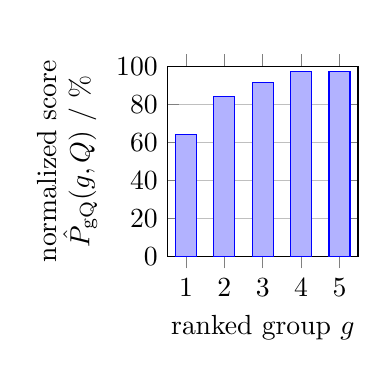
\begin{tikzpicture}[baseline]
\begin{axis}[
ybar, ymin=0, ymax=100,
xmin=1, xmax=5,
width=4cm, height=4cm,
symbolic x coords={1,2,3,4,5},
xtick=data,
xlabel={ranked group $g$},
ylabel={\parbox{9em}{\centering normalized score \\ $\hat{P}_{\rm gQ}(g,Q)$ / \%}},
ymajorgrids=true,
enlarge x limits=0.12,
bar width=0.266667cm,
]
\addplot coordinates {
(1,64.2857)
(2,84.2857)
(3,91.3669)
(4,97.1429)
(5,97.1223)
};
\end{axis}
\end{tikzpicture}

\end{minipage}

\vspace{1cm}
\noindent
\begin{minipage}{\textwidth}
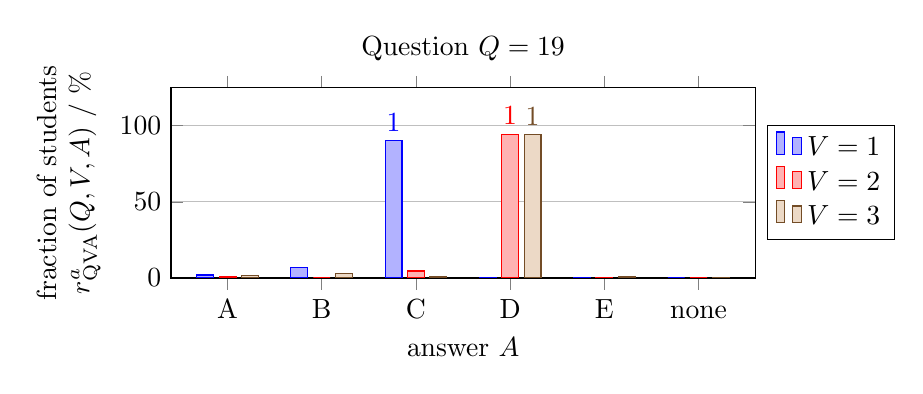
\begin{tikzpicture}[baseline]
\begin{axis}[
title={Question $Q = 19$},
ybar, ymin=0, ymax=100,
width=9cm, height=4cm,
xlabel={answer $A$},
ylabel={\parbox{9em}{\centering fraction of students \\ $r^a_{\rm QVA}(Q,V,A)$ / \%}},
symbolic x coords={A,B,C,D,E,none},
xticklabels={A,B,C,D,E,\vphantom{A}none},
xtick=data,
ymajorgrids=true,
enlarge x limits=0.12,
enlarge y limits={upper,value=0.25},
legend style={at={(1.02,0.5)},anchor=west},
bar width=0.214286cm,
point meta=explicit,
nodes near coords={\pgfmathfloatifflags{\pgfplotspointmeta}{0}{}{\pgfmathprintnumber{\pgfplotspointmeta}}},
]
\addplot coordinates {
(A,2) [0]
(B,7) [0]
(C,90) [1]
(D,0.5) [0]
(E,0.5) [0]
(none,0) [0]
};
\addplot coordinates {
(A,0.917431) [0]
(B,0) [0]
(C,4.58716) [0]
(D,94.0367) [1]
(E,0.458716) [0]
(none,0) [0]
};
\addplot coordinates {
(A,1.42857) [0]
(B,2.85714) [0]
(C,0.714286) [0]
(D,93.9286) [1]
(E,0.714286) [0]
(none,0.357143) [0]
};
\legend{$V = 1$,$V = 2$,$V = 3$};
\end{axis}
\end{tikzpicture}
\hfill
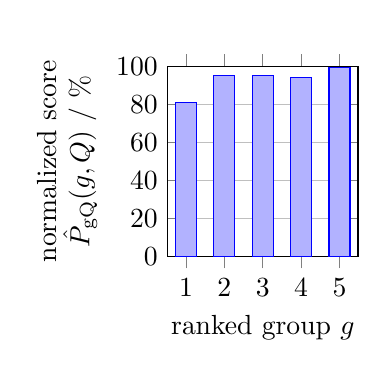
\begin{tikzpicture}[baseline]
\begin{axis}[
ybar, ymin=0, ymax=100,
xmin=1, xmax=5,
width=4cm, height=4cm,
symbolic x coords={1,2,3,4,5},
xtick=data,
xlabel={ranked group $g$},
ylabel={\parbox{9em}{\centering normalized score \\ $\hat{P}_{\rm gQ}(g,Q)$ / \%}},
ymajorgrids=true,
enlarge x limits=0.12,
bar width=0.266667cm,
]
\addplot coordinates {
(1,80.7143)
(2,95)
(3,94.964)
(4,94.2857)
(5,99.2806)
};
\end{axis}
\end{tikzpicture}

\end{minipage}

\vspace{1cm}
\noindent
\begin{minipage}{\textwidth}
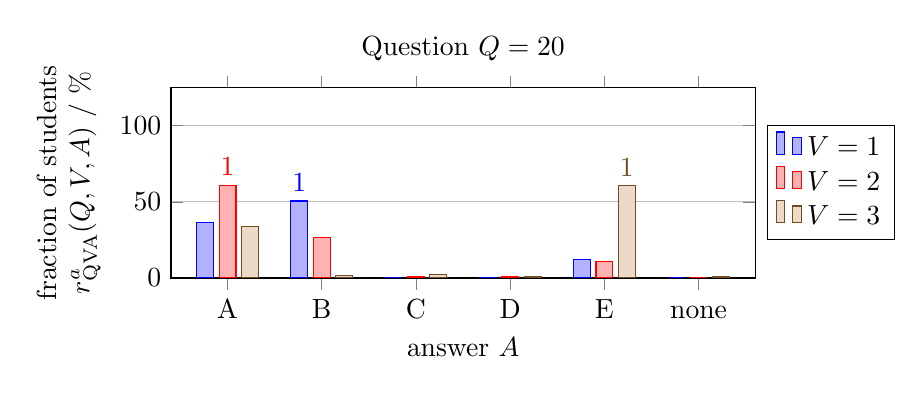
\begin{tikzpicture}[baseline]
\begin{axis}[
title={Question $Q = 20$},
ybar, ymin=0, ymax=100,
width=9cm, height=4cm,
xlabel={answer $A$},
ylabel={\parbox{9em}{\centering fraction of students \\ $r^a_{\rm QVA}(Q,V,A)$ / \%}},
symbolic x coords={A,B,C,D,E,none},
xticklabels={A,B,C,D,E,\vphantom{A}none},
xtick=data,
ymajorgrids=true,
enlarge x limits=0.12,
enlarge y limits={upper,value=0.25},
legend style={at={(1.02,0.5)},anchor=west},
bar width=0.214286cm,
point meta=explicit,
nodes near coords={\pgfmathfloatifflags{\pgfplotspointmeta}{0}{}{\pgfmathprintnumber{\pgfplotspointmeta}}},
]
\addplot coordinates {
(A,36.5591) [0]
(B,50.5376) [1]
(C,0) [0]
(D,0.537634) [0]
(E,12.3656) [0]
(none,0) [0]
};
\addplot coordinates {
(A,60.6178) [1]
(B,26.6409) [0]
(C,1.1583) [0]
(D,0.772201) [0]
(E,10.8108) [0]
(none,0) [0]
};
\addplot coordinates {
(A,33.9921) [0]
(B,1.58103) [0]
(C,2.37154) [0]
(D,0.790514) [0]
(E,60.4743) [1]
(none,0.790514) [0]
};
\legend{$V = 1$,$V = 2$,$V = 3$};
\end{axis}
\end{tikzpicture}
\hfill
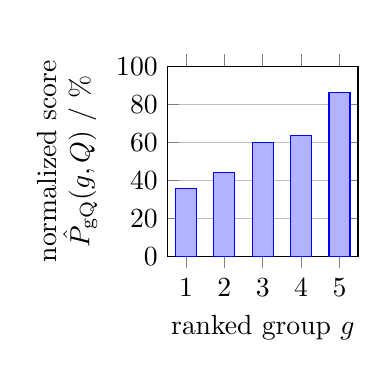
\begin{tikzpicture}[baseline]
\begin{axis}[
ybar, ymin=0, ymax=100,
xmin=1, xmax=5,
width=4cm, height=4cm,
symbolic x coords={1,2,3,4,5},
xtick=data,
xlabel={ranked group $g$},
ylabel={\parbox{9em}{\centering normalized score \\ $\hat{P}_{\rm gQ}(g,Q)$ / \%}},
ymajorgrids=true,
enlarge x limits=0.12,
bar width=0.266667cm,
]
\addplot coordinates {
(1,35.7143)
(2,44.2857)
(3,59.7122)
(4,63.5714)
(5,86.3309)
};
\end{axis}
\end{tikzpicture}

\end{minipage}

\vspace{1cm}
\noindent
\begin{minipage}{\textwidth}
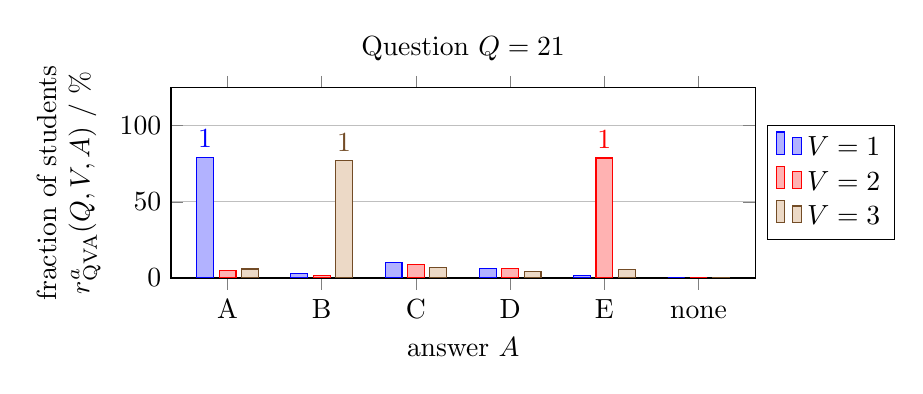
\begin{tikzpicture}[baseline]
\begin{axis}[
title={Question $Q = 21$},
ybar, ymin=0, ymax=100,
width=9cm, height=4cm,
xlabel={answer $A$},
ylabel={\parbox{9em}{\centering fraction of students \\ $r^a_{\rm QVA}(Q,V,A)$ / \%}},
symbolic x coords={A,B,C,D,E,none},
xticklabels={A,B,C,D,E,\vphantom{A}none},
xtick=data,
ymajorgrids=true,
enlarge x limits=0.12,
enlarge y limits={upper,value=0.25},
legend style={at={(1.02,0.5)},anchor=west},
bar width=0.214286cm,
point meta=explicit,
nodes near coords={\pgfmathfloatifflags{\pgfplotspointmeta}{0}{}{\pgfmathprintnumber{\pgfplotspointmeta}}},
]
\addplot coordinates {
(A,79.1209) [1]
(B,2.74725) [0]
(C,10.4396) [0]
(D,6.04396) [0]
(E,1.64835) [0]
(none,0) [0]
};
\addplot coordinates {
(A,4.67626) [0]
(B,1.43885) [0]
(C,8.99281) [0]
(D,6.11511) [0]
(E,78.777) [1]
(none,0) [0]
};
\addplot coordinates {
(A,5.88235) [0]
(B,76.8908) [1]
(C,7.14286) [0]
(D,4.20168) [0]
(E,5.46218) [0]
(none,0.420168) [0]
};
\legend{$V = 1$,$V = 2$,$V = 3$};
\end{axis}
\end{tikzpicture}
\hfill
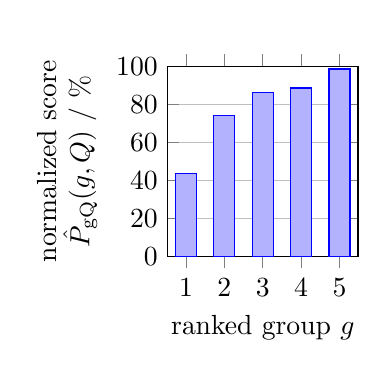
\begin{tikzpicture}[baseline]
\begin{axis}[
ybar, ymin=0, ymax=100,
xmin=1, xmax=5,
width=4cm, height=4cm,
symbolic x coords={1,2,3,4,5},
xtick=data,
xlabel={ranked group $g$},
ylabel={\parbox{9em}{\centering normalized score \\ $\hat{P}_{\rm gQ}(g,Q)$ / \%}},
ymajorgrids=true,
enlarge x limits=0.12,
bar width=0.266667cm,
]
\addplot coordinates {
(1,43.5714)
(2,74.2857)
(3,86.3309)
(4,88.5714)
(5,98.5612)
};
\end{axis}
\end{tikzpicture}

\end{minipage}

\vspace{1cm}
\noindent
\begin{minipage}{\textwidth}
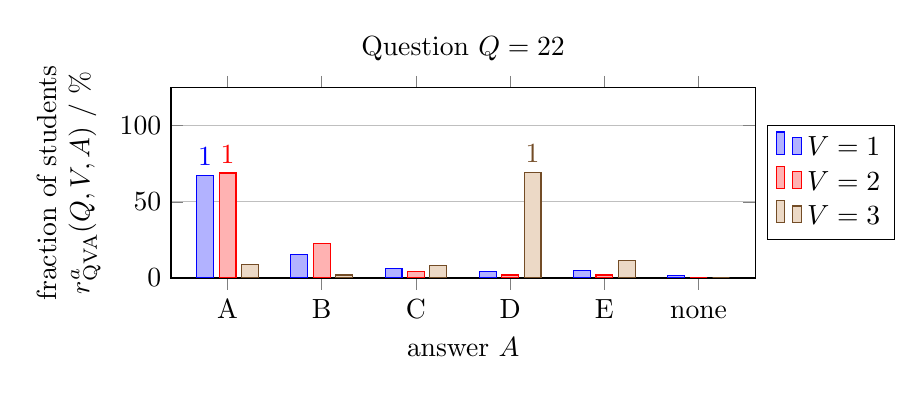
\begin{tikzpicture}[baseline]
\begin{axis}[
title={Question $Q = 22$},
ybar, ymin=0, ymax=100,
width=9cm, height=4cm,
xlabel={answer $A$},
ylabel={\parbox{9em}{\centering fraction of students \\ $r^a_{\rm QVA}(Q,V,A)$ / \%}},
symbolic x coords={A,B,C,D,E,none},
xticklabels={A,B,C,D,E,\vphantom{A}none},
xtick=data,
ymajorgrids=true,
enlarge x limits=0.12,
enlarge y limits={upper,value=0.25},
legend style={at={(1.02,0.5)},anchor=west},
bar width=0.214286cm,
point meta=explicit,
nodes near coords={\pgfmathfloatifflags{\pgfplotspointmeta}{0}{}{\pgfmathprintnumber{\pgfplotspointmeta}}},
]
\addplot coordinates {
(A,67.234) [1]
(B,15.3191) [0]
(C,6.38298) [0]
(D,4.25532) [0]
(E,5.10638) [0]
(none,1.70213) [0]
};
\addplot coordinates {
(A,68.932) [1]
(B,22.8155) [0]
(C,4.36893) [0]
(D,1.94175) [0]
(E,1.94175) [0]
(none,0) [0]
};
\addplot coordinates {
(A,8.94942) [0]
(B,1.94553) [0]
(C,8.17121) [0]
(D,69.2607) [1]
(E,11.6732) [0]
(none,0) [0]
};
\legend{$V = 1$,$V = 2$,$V = 3$};
\end{axis}
\end{tikzpicture}
\hfill
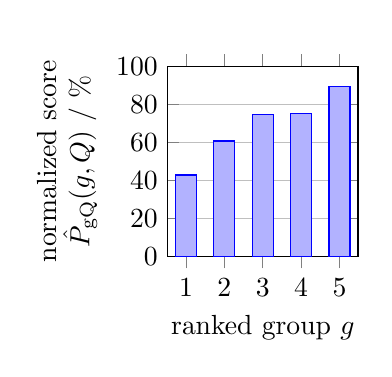
\begin{tikzpicture}[baseline]
\begin{axis}[
ybar, ymin=0, ymax=100,
xmin=1, xmax=5,
width=4cm, height=4cm,
symbolic x coords={1,2,3,4,5},
xtick=data,
xlabel={ranked group $g$},
ylabel={\parbox{9em}{\centering normalized score \\ $\hat{P}_{\rm gQ}(g,Q)$ / \%}},
ymajorgrids=true,
enlarge x limits=0.12,
bar width=0.266667cm,
]
\addplot coordinates {
(1,42.8571)
(2,60.7143)
(3,74.8201)
(4,75)
(5,89.2086)
};
\end{axis}
\end{tikzpicture}

\end{minipage}

\vspace{1cm}
\noindent
\begin{minipage}{\textwidth}
\begin{tikzpicture}[baseline]
\begin{axis}[
title={Question $Q = 23$},
ybar, ymin=0, ymax=100,
width=9cm, height=4cm,
xlabel={answer $A$},
ylabel={\parbox{9em}{\centering fraction of students \\ $r^a_{\rm QVA}(Q,V,A)$ / \%}},
symbolic x coords={A,B,C,D,E,none},
xticklabels={A,B,C,D,E,\vphantom{A}none},
xtick=data,
ymajorgrids=true,
enlarge x limits=0.12,
enlarge y limits={upper,value=0.25},
legend style={at={(1.02,0.5)},anchor=west},
bar width=0.214286cm,
point meta=explicit,
nodes near coords={\pgfmathfloatifflags{\pgfplotspointmeta}{0}{}{\pgfmathprintnumber{\pgfplotspointmeta}}},
]
\addplot coordinates {
(A,3.93443) [0]
(B,0) [0]
(C,0) [0]
(D,0) [0]
(E,95.7377) [1]
(none,0.327869) [0]
};
\addplot coordinates {
(A,3.30789) [0]
(B,0.254453) [0]
(C,0.508906) [0]
(D,0) [0]
(E,95.6743) [1]
(none,0.254453) [0]
};
\legend{$V = 1$,$V = 2$};
\end{axis}
\end{tikzpicture}
\hfill
\begin{tikzpicture}[baseline]
\begin{axis}[
ybar, ymin=0, ymax=100,
xmin=1, xmax=5,
width=4cm, height=4cm,
symbolic x coords={1,2,3,4,5},
xtick=data,
xlabel={ranked group $g$},
ylabel={\parbox{9em}{\centering normalized score \\ $\hat{P}_{\rm gQ}(g,Q)$ / \%}},
ymajorgrids=true,
enlarge x limits=0.12,
bar width=0.266667cm,
]
\addplot coordinates {
(1,95)
(2,91.4286)
(3,95.6835)
(4,96.4286)
(5,100)
};
\end{axis}
\end{tikzpicture}

\end{minipage}

\vspace{1cm}
\noindent
\begin{minipage}{\textwidth}
\begin{tikzpicture}[baseline]
\begin{axis}[
title={Question $Q = 24$},
ybar, ymin=0, ymax=100,
width=9cm, height=4cm,
xlabel={answer $A$},
ylabel={\parbox{9em}{\centering fraction of students \\ $r^a_{\rm QVA}(Q,V,A)$ / \%}},
symbolic x coords={A,B,C,D,E,none},
xticklabels={A,B,C,D,E,\vphantom{A}none},
xtick=data,
ymajorgrids=true,
enlarge x limits=0.12,
enlarge y limits={upper,value=0.25},
legend style={at={(1.02,0.5)},anchor=west},
bar width=0.214286cm,
point meta=explicit,
nodes near coords={\pgfmathfloatifflags{\pgfplotspointmeta}{0}{}{\pgfmathprintnumber{\pgfplotspointmeta}}},
]
\addplot coordinates {
(A,3.90071) [0]
(B,1.41844) [0]
(C,90.4255) [1]
(D,2.48227) [0]
(E,1.77305) [0]
(none,0) [0]
};
\addplot coordinates {
(A,3.84615) [0]
(B,1.68269) [0]
(C,93.5096) [1]
(D,0.480769) [0]
(E,0.240385) [0]
(none,0.240385) [0]
};
\legend{$V = 1$,$V = 2$};
\end{axis}
\end{tikzpicture}
\hfill
\begin{tikzpicture}[baseline]
\begin{axis}[
ybar, ymin=0, ymax=100,
xmin=1, xmax=5,
width=4cm, height=4cm,
symbolic x coords={1,2,3,4,5},
xtick=data,
xlabel={ranked group $g$},
ylabel={\parbox{9em}{\centering normalized score \\ $\hat{P}_{\rm gQ}(g,Q)$ / \%}},
ymajorgrids=true,
enlarge x limits=0.12,
bar width=0.266667cm,
]
\addplot coordinates {
(1,75.7143)
(2,92.8571)
(3,96.4029)
(4,98.5714)
(5,97.8417)
};
\end{axis}
\end{tikzpicture}

\end{minipage}

\vspace{1cm}
\noindent
\begin{minipage}{\textwidth}
\begin{tikzpicture}[baseline]
\begin{axis}[
title={Question $Q = 25$},
ybar, ymin=0, ymax=100,
width=9cm, height=4cm,
xlabel={answer $A$},
ylabel={\parbox{9em}{\centering fraction of students \\ $r^a_{\rm QVA}(Q,V,A)$ / \%}},
symbolic x coords={A,B,C,D,E,none},
xticklabels={A,B,C,D,E,\vphantom{A}none},
xtick=data,
ymajorgrids=true,
enlarge x limits=0.12,
enlarge y limits={upper,value=0.25},
legend style={at={(1.02,0.5)},anchor=west},
bar width=0.214286cm,
point meta=explicit,
nodes near coords={\pgfmathfloatifflags{\pgfplotspointmeta}{0}{}{\pgfmathprintnumber{\pgfplotspointmeta}}},
]
\addplot coordinates {
(A,3.89972) [0]
(B,13.649) [0]
(C,74.6518) [1]
(D,3.62117) [0]
(E,4.17827) [0]
(none,0) [0]
};
\addplot coordinates {
(A,88.4956) [1]
(B,5.60472) [0]
(C,0) [0]
(D,1.17994) [0]
(E,4.71976) [0]
(none,0) [0]
};
\legend{$V = 1$,$V = 2$};
\end{axis}
\end{tikzpicture}
\hfill
\begin{tikzpicture}[baseline]
\begin{axis}[
ybar, ymin=0, ymax=100,
xmin=1, xmax=5,
width=4cm, height=4cm,
symbolic x coords={1,2,3,4,5},
xtick=data,
xlabel={ranked group $g$},
ylabel={\parbox{9em}{\centering normalized score \\ $\hat{P}_{\rm gQ}(g,Q)$ / \%}},
ymajorgrids=true,
enlarge x limits=0.12,
bar width=0.266667cm,
]
\addplot coordinates {
(1,50.7143)
(2,79.2857)
(3,87.7698)
(4,90)
(5,99.2806)
};
\end{axis}
\end{tikzpicture}

\end{minipage}

\vspace{1cm}
\noindent
\begin{minipage}{\textwidth}
\begin{tikzpicture}[baseline]
\begin{axis}[
title={Question $Q = 26$},
ybar, ymin=0, ymax=100,
width=9cm, height=4cm,
xlabel={answer $A$},
ylabel={\parbox{9em}{\centering fraction of students \\ $r^a_{\rm QVA}(Q,V,A)$ / \%}},
symbolic x coords={A,B,C,D,E,none},
xticklabels={A,B,C,D,E,\vphantom{A}none},
xtick=data,
ymajorgrids=true,
enlarge x limits=0.12,
enlarge y limits={upper,value=0.25},
legend style={at={(1.02,0.5)},anchor=west},
bar width=0.214286cm,
point meta=explicit,
nodes near coords={\pgfmathfloatifflags{\pgfplotspointmeta}{0}{}{\pgfmathprintnumber{\pgfplotspointmeta}}},
]
\addplot coordinates {
(A,0) [0]
(B,7.54717) [0]
(C,75.9434) [1]
(D,7.54717) [0]
(E,8.96226) [0]
(none,0) [0]
};
\addplot coordinates {
(A,67.7165) [1]
(B,1.5748) [0]
(C,0.787402) [0]
(D,20.8661) [0]
(E,9.05512) [0]
(none,0) [0]
};
\addplot coordinates {
(A,15.0862) [0]
(B,10.7759) [0]
(C,44.3966) [1]
(D,14.2241) [0]
(E,15.0862) [0]
(none,0.431034) [0]
};
\legend{$V = 1$,$V = 2$,$V = 3$};
\end{axis}
\end{tikzpicture}
\hfill
\begin{tikzpicture}[baseline]
\begin{axis}[
ybar, ymin=0, ymax=100,
xmin=1, xmax=5,
width=4cm, height=4cm,
symbolic x coords={1,2,3,4,5},
xtick=data,
xlabel={ranked group $g$},
ylabel={\parbox{9em}{\centering normalized score \\ $\hat{P}_{\rm gQ}(g,Q)$ / \%}},
ymajorgrids=true,
enlarge x limits=0.12,
bar width=0.266667cm,
]
\addplot coordinates {
(1,28.5714)
(2,45)
(3,72.6619)
(4,77.8571)
(5,88.4892)
};
\end{axis}
\end{tikzpicture}

\end{minipage}

\vspace{1cm}
\noindent
\begin{minipage}{\textwidth}
\begin{tikzpicture}[baseline]
\begin{axis}[
title={Question $Q = 27$},
ybar, ymin=0, ymax=100,
width=9cm, height=4cm,
xlabel={answer $A$},
ylabel={\parbox{9em}{\centering fraction of students \\ $r^a_{\rm QVA}(Q,V,A)$ / \%}},
symbolic x coords={A,B,C,D,E,none},
xticklabels={A,B,C,D,E,\vphantom{A}none},
xtick=data,
ymajorgrids=true,
enlarge x limits=0.12,
enlarge y limits={upper,value=0.25},
legend style={at={(1.02,0.5)},anchor=west},
bar width=0.214286cm,
point meta=explicit,
nodes near coords={\pgfmathfloatifflags{\pgfplotspointmeta}{0}{}{\pgfmathprintnumber{\pgfplotspointmeta}}},
]
\addplot coordinates {
(A,82.3322) [1]
(B,4.24028) [0]
(C,10.2473) [0]
(D,1.41343) [0]
(E,1.76678) [0]
(none,0) [0]
};
\addplot coordinates {
(A,77.9343) [1]
(B,3.75587) [0]
(C,14.0845) [0]
(D,0.469484) [0]
(E,3.75587) [0]
(none,0) [0]
};
\addplot coordinates {
(A,87.1287) [1]
(B,8.41584) [0]
(C,2.47525) [0]
(D,1.48515) [0]
(E,0.49505) [0]
(none,0) [0]
};
\legend{$V = 1$,$V = 2$,$V = 3$};
\end{axis}
\end{tikzpicture}
\hfill
\begin{tikzpicture}[baseline]
\begin{axis}[
ybar, ymin=0, ymax=100,
xmin=1, xmax=5,
width=4cm, height=4cm,
symbolic x coords={1,2,3,4,5},
xtick=data,
xlabel={ranked group $g$},
ylabel={\parbox{9em}{\centering normalized score \\ $\hat{P}_{\rm gQ}(g,Q)$ / \%}},
ymajorgrids=true,
enlarge x limits=0.12,
bar width=0.266667cm,
]
\addplot coordinates {
(1,57.1429)
(2,75)
(3,85.6115)
(4,97.1429)
(5,97.1223)
};
\end{axis}
\end{tikzpicture}

\end{minipage}

\vspace{1cm}
\noindent
\begin{minipage}{\textwidth}
\begin{tikzpicture}[baseline]
\begin{axis}[
title={Question $Q = 28$},
ybar, ymin=0, ymax=100,
width=9cm, height=4cm,
xlabel={answer $A$},
ylabel={\parbox{9em}{\centering fraction of students \\ $r^a_{\rm QVA}(Q,V,A)$ / \%}},
symbolic x coords={A,B,C,D,E,none},
xticklabels={A,B,C,D,E,\vphantom{A}none},
xtick=data,
ymajorgrids=true,
enlarge x limits=0.12,
enlarge y limits={upper,value=0.25},
legend style={at={(1.02,0.5)},anchor=west},
bar width=0.214286cm,
point meta=explicit,
nodes near coords={\pgfmathfloatifflags{\pgfplotspointmeta}{0}{}{\pgfmathprintnumber{\pgfplotspointmeta}}},
]
\addplot coordinates {
(A,1.28535) [0]
(B,75.5784) [1]
(C,1.28535) [0]
(D,20.5656) [0]
(E,1.28535) [0]
(none,0) [0]
};
\addplot coordinates {
(A,10.356) [0]
(B,41.4239) [0]
(C,27.8317) [0]
(D,0.970874) [0]
(E,19.4175) [1]
(none,0) [0]
};
\legend{$V = 1$,$V = 2$};
\end{axis}
\end{tikzpicture}
\hfill
\begin{tikzpicture}[baseline]
\begin{axis}[
ybar, ymin=0, ymax=100,
xmin=1, xmax=5,
width=4cm, height=4cm,
symbolic x coords={1,2,3,4,5},
xtick=data,
xlabel={ranked group $g$},
ylabel={\parbox{9em}{\centering normalized score \\ $\hat{P}_{\rm gQ}(g,Q)$ / \%}},
ymajorgrids=true,
enlarge x limits=0.12,
bar width=0.266667cm,
]
\addplot coordinates {
(1,39.2857)
(2,47.8571)
(3,46.0432)
(4,52.8571)
(5,67.6259)
};
\end{axis}
\end{tikzpicture}

\end{minipage}

\vspace{1cm}
\noindent
\begin{minipage}{\textwidth}
\begin{tikzpicture}[baseline]
\begin{axis}[
title={Question $Q = 29$},
ybar, ymin=0, ymax=100,
width=9cm, height=4cm,
xlabel={answer $A$},
ylabel={\parbox{9em}{\centering fraction of students \\ $r^a_{\rm QVA}(Q,V,A)$ / \%}},
symbolic x coords={A,B,C,D,E,none},
xticklabels={A,B,C,D,E,\vphantom{A}none},
xtick=data,
ymajorgrids=true,
enlarge x limits=0.12,
enlarge y limits={upper,value=0.25},
legend style={at={(1.02,0.5)},anchor=west},
bar width=0.214286cm,
point meta=explicit,
nodes near coords={\pgfmathfloatifflags{\pgfplotspointmeta}{0}{}{\pgfmathprintnumber{\pgfplotspointmeta}}},
]
\addplot coordinates {
(A,18.3206) [1]
(B,75.3181) [1]
(C,3.30789) [1]
(D,1.27226) [1]
(E,1.52672) [1]
(none,0.254453) [0]
};
\addplot coordinates {
(A,22.2951) [1]
(B,68.5246) [1]
(C,2.62295) [1]
(D,5.2459) [1]
(E,0.983607) [1]
(none,0.327869) [0]
};
\legend{$V = 1$,$V = 2$};
\end{axis}
\end{tikzpicture}
\hfill
\begin{tikzpicture}[baseline]
\begin{axis}[
ybar, ymin=0, ymax=100,
xmin=1, xmax=5,
width=4cm, height=4cm,
symbolic x coords={1,2,3,4,5},
xtick=data,
xlabel={ranked group $g$},
ylabel={\parbox{9em}{\centering normalized score \\ $\hat{P}_{\rm gQ}(g,Q)$ / \%}},
ymajorgrids=true,
enlarge x limits=0.12,
bar width=0.266667cm,
]
\addplot coordinates {
(1,99.2857)
(2,99.2857)
(3,100)
(4,100)
(5,100)
};
\end{axis}
\end{tikzpicture}

\end{minipage}

\vspace{1cm}
\noindent
\begin{minipage}{\textwidth}
\begin{tikzpicture}[baseline]
\begin{axis}[
title={Question $Q = 30$},
ybar, ymin=0, ymax=100,
width=9cm, height=4cm,
xlabel={answer $A$},
ylabel={\parbox{9em}{\centering fraction of students \\ $r^a_{\rm QVA}(Q,V,A)$ / \%}},
symbolic x coords={A,B,C,D,E,none},
xticklabels={A,B,C,D,E,\vphantom{A}none},
xtick=data,
ymajorgrids=true,
enlarge x limits=0.12,
enlarge y limits={upper,value=0.25},
legend style={at={(1.02,0.5)},anchor=west},
bar width=0.214286cm,
point meta=explicit,
nodes near coords={\pgfmathfloatifflags{\pgfplotspointmeta}{0}{}{\pgfmathprintnumber{\pgfplotspointmeta}}},
]
\addplot coordinates {
(A,10.5263) [1]
(B,7.45614) [1]
(C,12.2807) [1]
(D,67.1053) [1]
(E,2.19298) [1]
(none,0.438596) [0]
};
\addplot coordinates {
(A,4.91803) [1]
(B,8.19672) [1]
(C,40.5738) [1]
(D,45.082) [1]
(E,1.22951) [1]
(none,0) [0]
};
\addplot coordinates {
(A,15.9292) [1]
(B,20.7965) [1]
(C,9.73451) [1]
(D,50.885) [1]
(E,2.21239) [1]
(none,0.442478) [0]
};
\legend{$V = 1$,$V = 2$,$V = 3$};
\end{axis}
\end{tikzpicture}
\hfill
\begin{tikzpicture}[baseline]
\begin{axis}[
ybar, ymin=0, ymax=100,
xmin=1, xmax=5,
width=4cm, height=4cm,
symbolic x coords={1,2,3,4,5},
xtick=data,
xlabel={ranked group $g$},
ylabel={\parbox{9em}{\centering normalized score \\ $\hat{P}_{\rm gQ}(g,Q)$ / \%}},
ymajorgrids=true,
enlarge x limits=0.12,
bar width=0.266667cm,
]
\addplot coordinates {
(1,99.2857)
(2,99.2857)
(3,100)
(4,100)
(5,100)
};
\end{axis}
\end{tikzpicture}

\end{minipage}

\end{document}
